% !TeX spellcheck = en_US
\lstset{
    basicstyle=\ttfamily\small,
    breaklines=true,
    numbers=left,
    numberstyle=\tiny,
    stepnumber=1,
    numbersep=5pt,
    %backgroundcolor=\color{gray!10},
    frame=lr,
    %captionpos=b,
    tabsize=2,
    keepspaces=true,
    showspaces=false,
    showstringspaces=false,
    showtabs=false,
    keywordstyle=\bfseries,
    commentstyle=\itshape\color{gray},
    stringstyle=\ttfamily\color{darkgray},
    lineskip=0.1em  % Add space between lines
}

\chapter{Evaluation}
\label{chap:evaluation}

This chapter presents a comprehensive evaluation of our smart home chatbot prototype. We begin by outlining our study design, which employs the \gls{gqm} paradigm to assess the chatbot. The evaluation process combines quantitative analysis of model performance with a user study to gather both objective metrics and subjective feedback. We then detail our evaluation methodology, including the selection of language models, creation of an evaluation dataset, and the metrics used to assess performance. The results section presents our findings from both the model evaluation and user study. Finally, we discuss these results, interpreting their implications for the effectiveness of our chatbot and identifying areas for future improvement. This multi-faceted approach provides a thorough understanding of our prototype's strengths and limitations.

\section{Study Design}
In this section we want to provide the base study design we came up.
The design of our evaluation was gathered through clearly defining the goals of the evaluation and coming to measurable metrics in the end via the top-down \gls{gqm} approach.
Our approach consists of three main goals: assessing the accuracy, the user experience and the explainability of the developed smart home chatbot.
Based on this we developed the whole evaluation process which consists of a \gls{llm} evaluation approach for the accuracy and a user study for the other two goals.
Details are provided later within this chapter.

\subsection{Goal Question Metric Paradigm}
The \gls{gqm} paradigm according to \citet{caldiera1994goal} provides a structured approach to evaluate different works in the area of Software Engineering and therefore is also suitable for evaluating various aspects of the smart home chatbot. 
Our evaluation framework consists of three primary goals, each addressing a specific area of interest: accuracy, user experience, and explainability.
This framework is shown in \cref{fig:gqm}

\textbf{Goal 1: Assess the Accuracy of the Smart Home Chatbot}

The first goal focuses on determining how accurately the chatbot can understand and respond to user commands. To achieve this, several questions are formulated:

\begin{itemize}
    \item \textbf{Q1: How accurate are the natural language answers of the language model?}
    \item \textbf{Q2: How accurate are the \gls{json} responses of the language model?}
\end{itemize}

To answer these questions, relevant metrics are identified. Semantic similarity measures are used to evaluate the natural language responses, potentially incorporating other related metrics to ensure comprehensive assessment. \gls{json} accuracy metrics are employed to evaluate the precision of the chatbot's structured responses. A combined metric of semantic similarity and JSON accuracy provides a holistic view of the chatbot's overall accuracy.

\textbf{Goal 2: Evaluate the User Experience of the Smart Home Chatbot}

The second goal is to understand the users' interaction experience with the chatbot. This involves evaluating how intuitive and satisfactory the chatbot is in performing tasks. The questions under this goal include:

\begin{itemize}
    \item \textbf{Q1: Are typical tasks easy to achieve?}
    \item \textbf{Q2: How satisfied are users with the chatbot's performance?}
    \item \textbf{Q3: What could be improved?}
    \item \textbf{Q4: Does the chatbot add to existing functionality of typical smart home applications?}
\end{itemize}

The metrics for these questions involve measuring task completion time, the number of attempts, and the success rate of task completion. User satisfaction is gauged through questionnaires administered after the experiment. These questionnaires assess various aspects of the user experience, including ease of use, overall satisfaction, and areas for improvement.

\textbf{Goal 3: Assess the Explainability of the Smart Home Chatbot}

The third goal addresses how well the chatbot can explain its actions and decisions to users, which is crucial for building trust and usability. The questions related to this goal are:

\begin{itemize}
    \item \textbf{Q1: How clear and understandable are the chatbot's explanations?}
    \item \textbf{Q2: What could be improved?}
\end{itemize}

To measure the explainability, semi-structured interviews are conducted after the experiment. These interviews delve into the clarity, transparency, and usefulness of the explanations provided by the chatbot, allowing for detailed qualitative feedback from users.

\begin{figure}[h]
    \centering
    \captionsetup{justification=centering}
    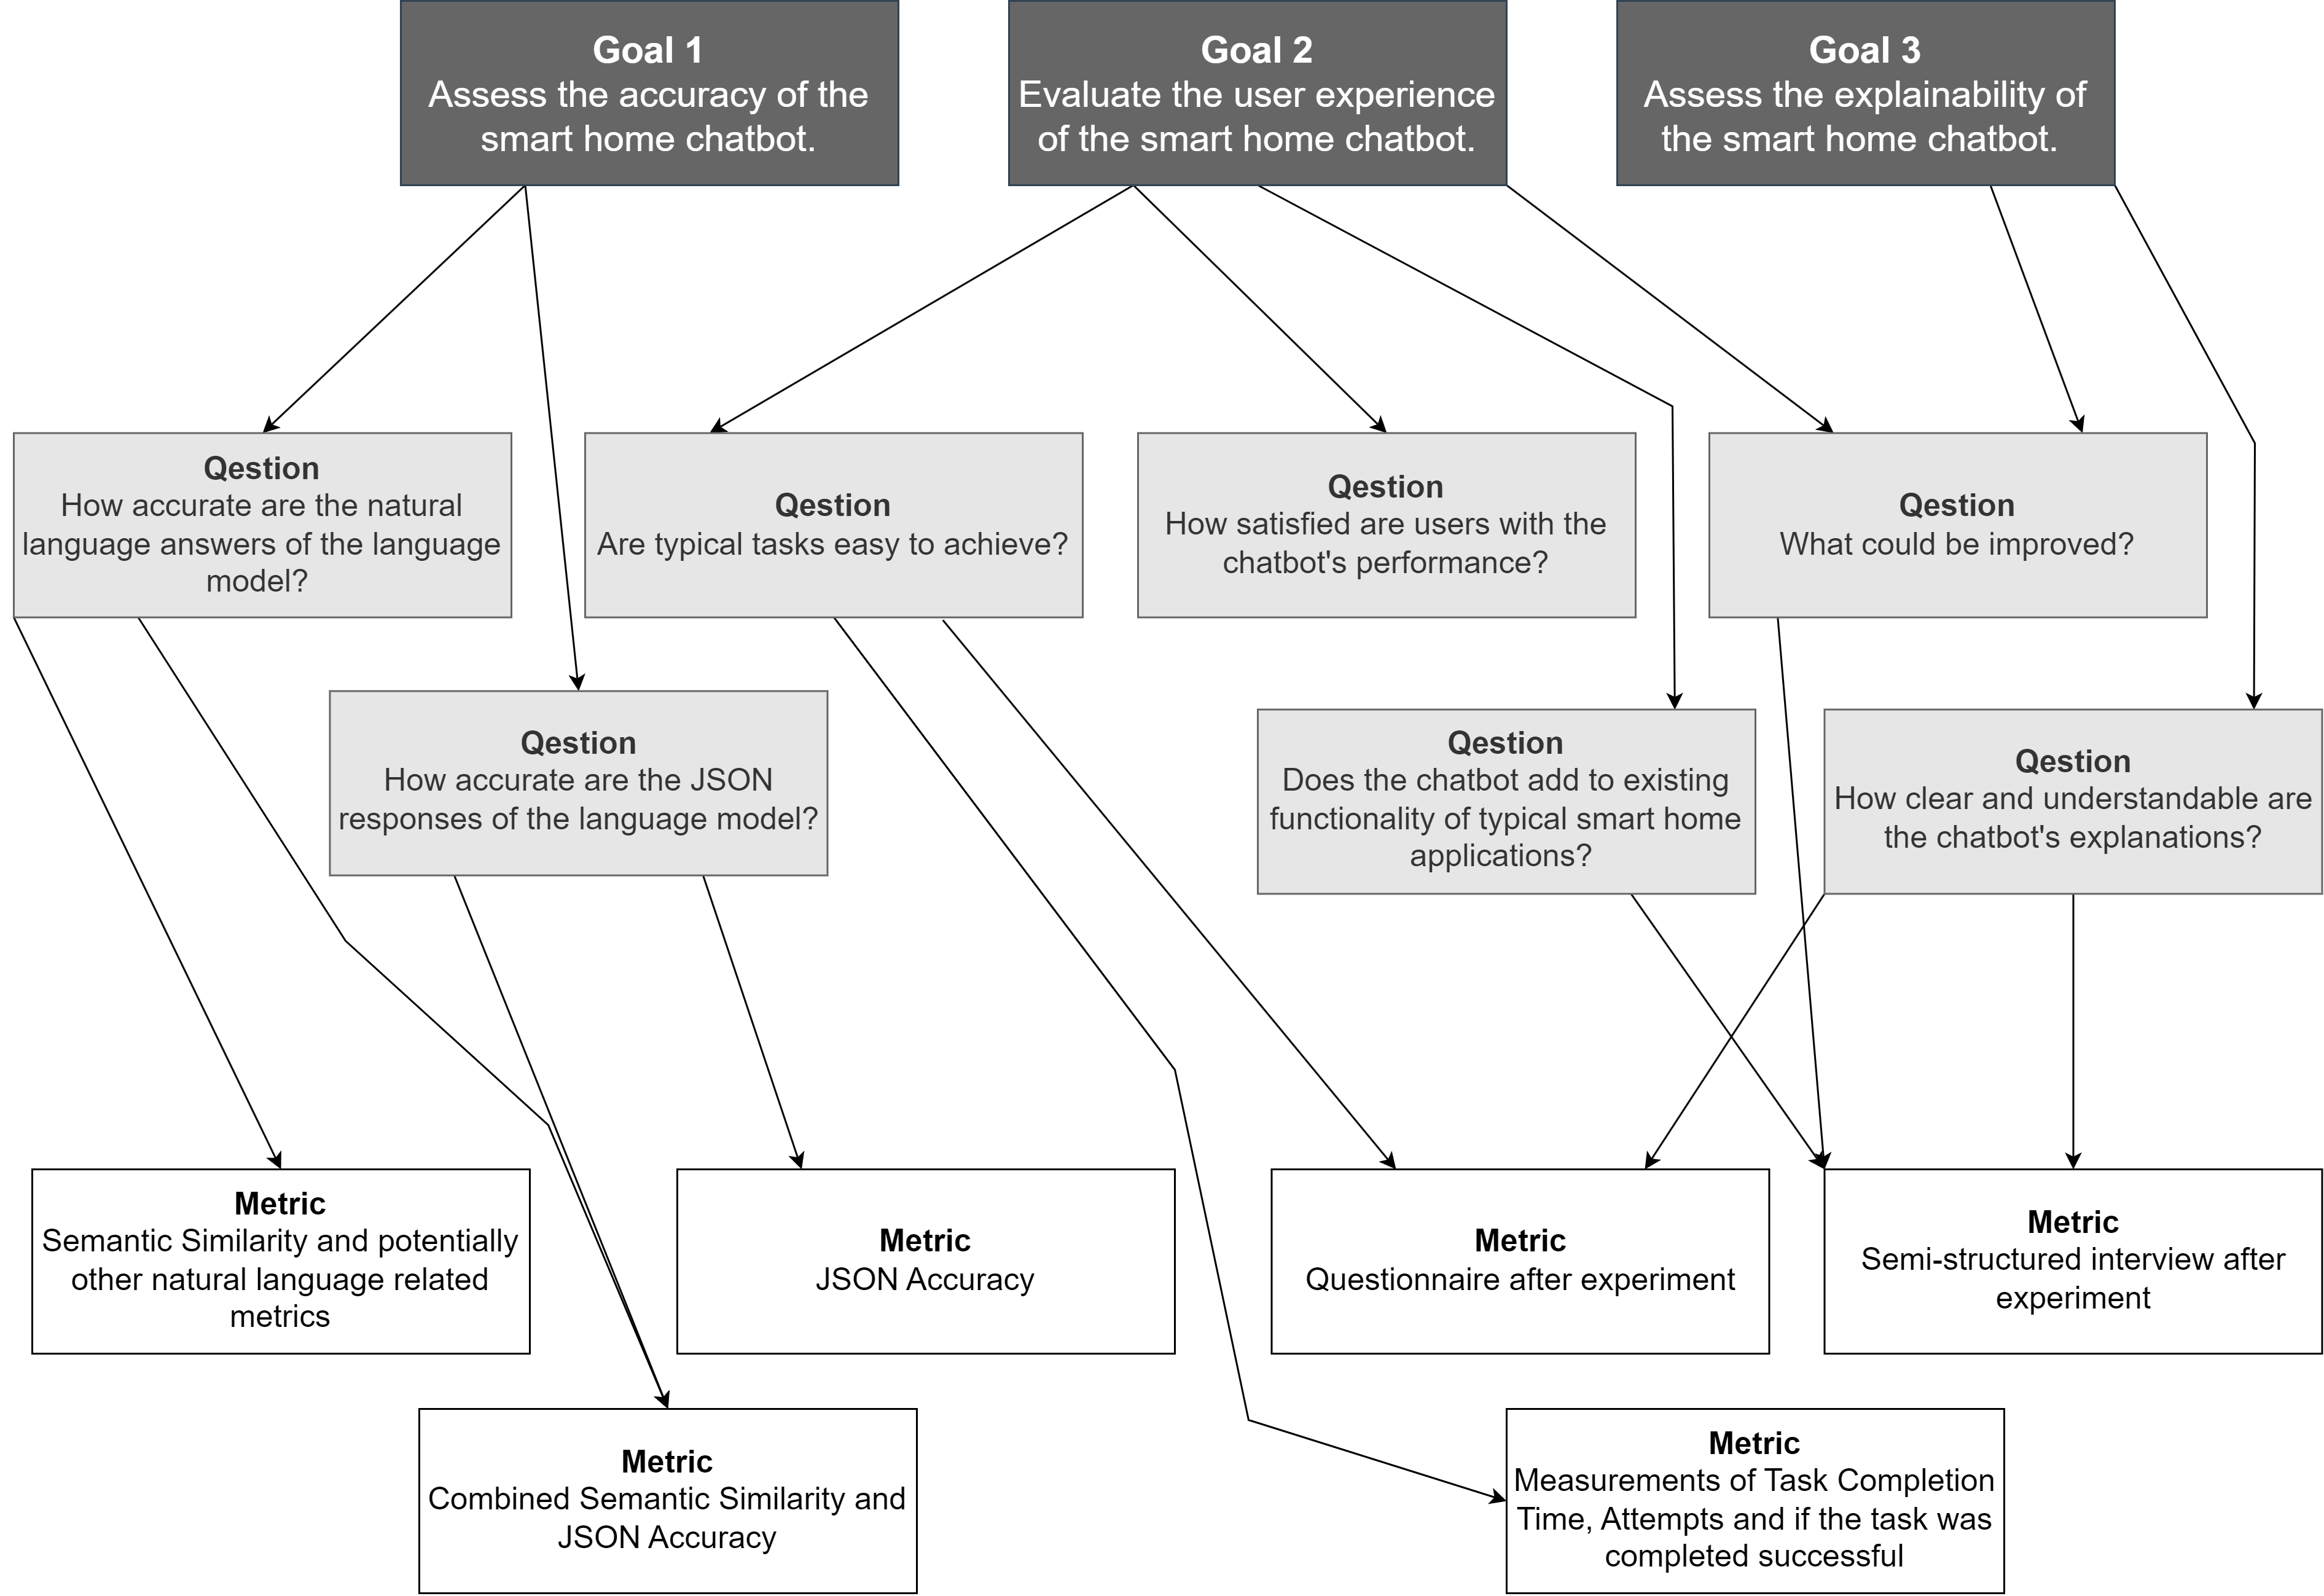
\includegraphics[width=0.98\textwidth]{graphics/gqm.png}
    \caption{Visualized Goal Question Metric}
    \label{fig:gqm}
\end{figure}
\begin{figure}[h]
    \centering
    \captionsetup{justification=centering}
    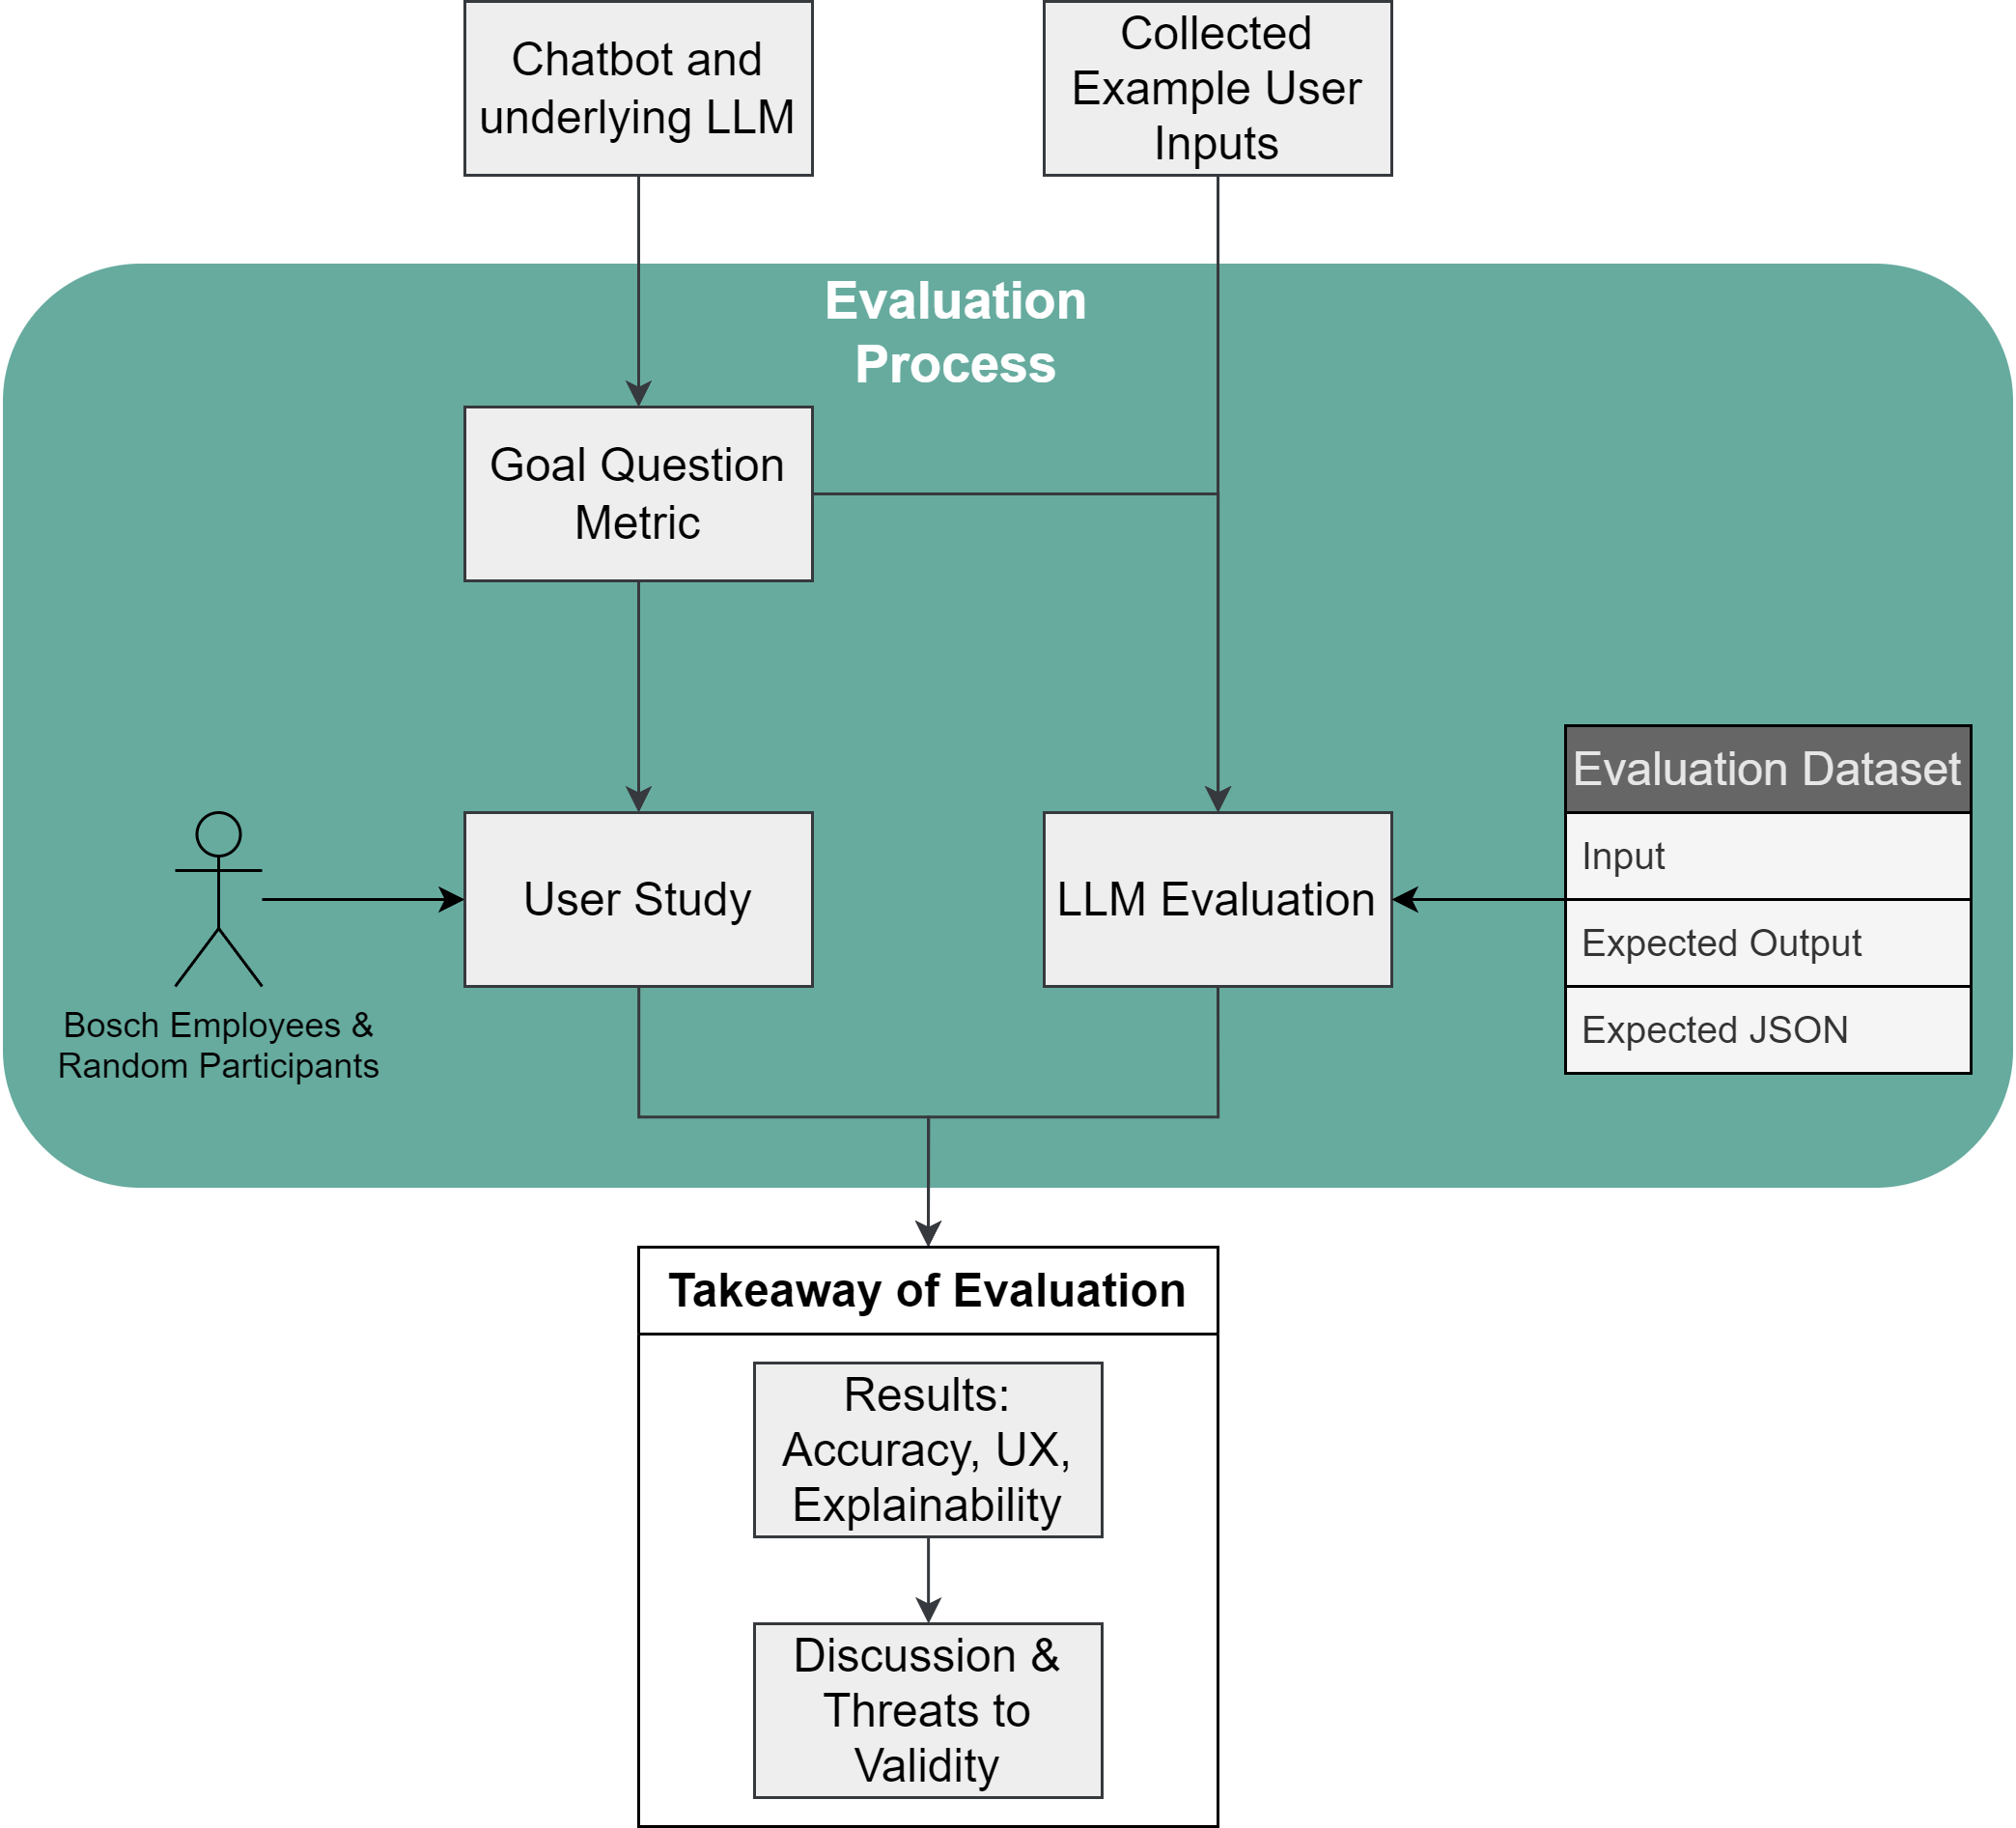
\includegraphics[width=0.75\textwidth]{graphics/eval-process.png}
    \caption{The Evaluation Process, Visualized}
    \label{fig:evalprocess}
\end{figure}

\subsection{Resulting Evaluation Process}
A Visualization of our evaluation process can be seen in \cref{fig:evalprocess}
Based on the obtained \gls{gqm}, the evaluation can be split into two parts: evaluating the model performance and a user study for examining User Experience and Explainability.
Besides the developed protoype chatbot the obtained sample user inputs can be greatly used in the evaluation process.
They could be used to construct the dataset that was essential for the evaluation of the language model.
This evaluation dataset contains for each sample input an expected natural language output and an eventually expected \gls{json} to measure both the accuracy of the output the user sees and the constructed \gls{json} that is used for further actions in the smart home system.

The other part is the user study in which users have a setup of devices that are supported by our prototype and receive a list of tasks in which the success should be measured and afterwards a questionnaire and a semi-structured interview are used to answer the questions regarding Goal 2 and 3 in the defined \gls{gqm}

Based on these two parts, the takeaway of this thesis can be received and constructed.
The results emerge directly as an output from the model evaluation and the user study when combined with quantitative and qualitative methods.

Based on this and the detailed evaluation setup the results can be discussed and threats to validity be debated.


\section{Model Performance}
\label{sec:modelperform}
This section details our approach to evaluating the performance of language models for our smart home chatbot. We describe the hardware setup and model selection process, explain the construction of our evaluation dataset, and outline the metrics used to assess both semantic similarity and \gls{json} accuracy. This evaluation framework allows us to compare different model iterations and identify the most suitable configuration for our chatbot prototype.

\subsection{Hardware and Language Models used}
\label{subsec:hardware-llm}
The hardware setup was the same as described in \cref{subsec:modelcust} since it is very fast for the model sizes we wanted to test as also explained in the same section.
For measuring the model performance there was no need to have a setup of smart home devices since when the outputed \gls{json} of the model is correct the correct action will be triggered in the underlying system.
The language models we selected for evaluation are also described in \cref{subsec:modelcust}.
We pre-filtered these models based on three selected typical user interactions from the evaluation dataset we created. If a model was not able to answer with a suitable \gls{json} or did not even understand the structure of the message history provided we excluded it from further evaluation with the whole dataset since it would not be worth investing the resources for it.
Only the llama3 model has passed this test (with two version: the normal 8b parameters model and the instruct version of it) and is therefore included in the further evaluation. The other models were not able to answer based on the device list provided with each user request. They usually answered with phrases like ``I can't find a device named 'TV'.''

\subsection{Evaluation Dataset}
To assess the performance and capabilities of our smart home chatbot, we developed a comprehensive evaluation dataset with a total of 80 entries. This dataset is designed to simulate realistic user interactions and test the chatbot's ability to understand context, control devices, and provide informative responses.
The evaluation dataset consists of a series of input-output pairs, where each input represents a chat history and the output represents the expected response from the chatbot. 
In creating the inputs for our evaluation dataset, we leveraged the user inputs collected during our earlier survey (as described in Section 4.4). These real-world examples provided authentic phrasing and diverse query formulations typical of smart home users. We adapted and expanded upon these collected inputs to ensure they aligned with our specific test scenarios and device setups. This approach allowed us to create a more realistic and challenging evaluation dataset, closely mimicking the variety of natural language inputs a smart home chatbot would encounter in practical use.
The structure of each entry in the dataset is as follows:

\begin{enumerate}
    \item Input: A chat history containing a minimum of two messages from the user. The first message always includes a device list that provides crucial context about the user's smart home environment. For details on the device list structure, refer to \cref{sec:req-building}.
    \item Expected Output: A natural language response that the chatbot is expected to generate based on the given chat history.
    \item Expected \gls{json}: A \gls{json} object representing the action the chatbot should take, if any. The \gls{json} includes only the necessary keys for each action:
    \begin{itemize}
    \item For 'turn-on' or 'turn-off' actions: 'action' and 'deviceID'
    \item For 'change-temperature' action: 'action', 'deviceID', and 'value'
    \item If no action is necessary, the expected \gls{json} is ``None''
    \end{itemize}
    \end{enumerate}

\begin{table}[htb]
    \centering
    \makebox[\textwidth]{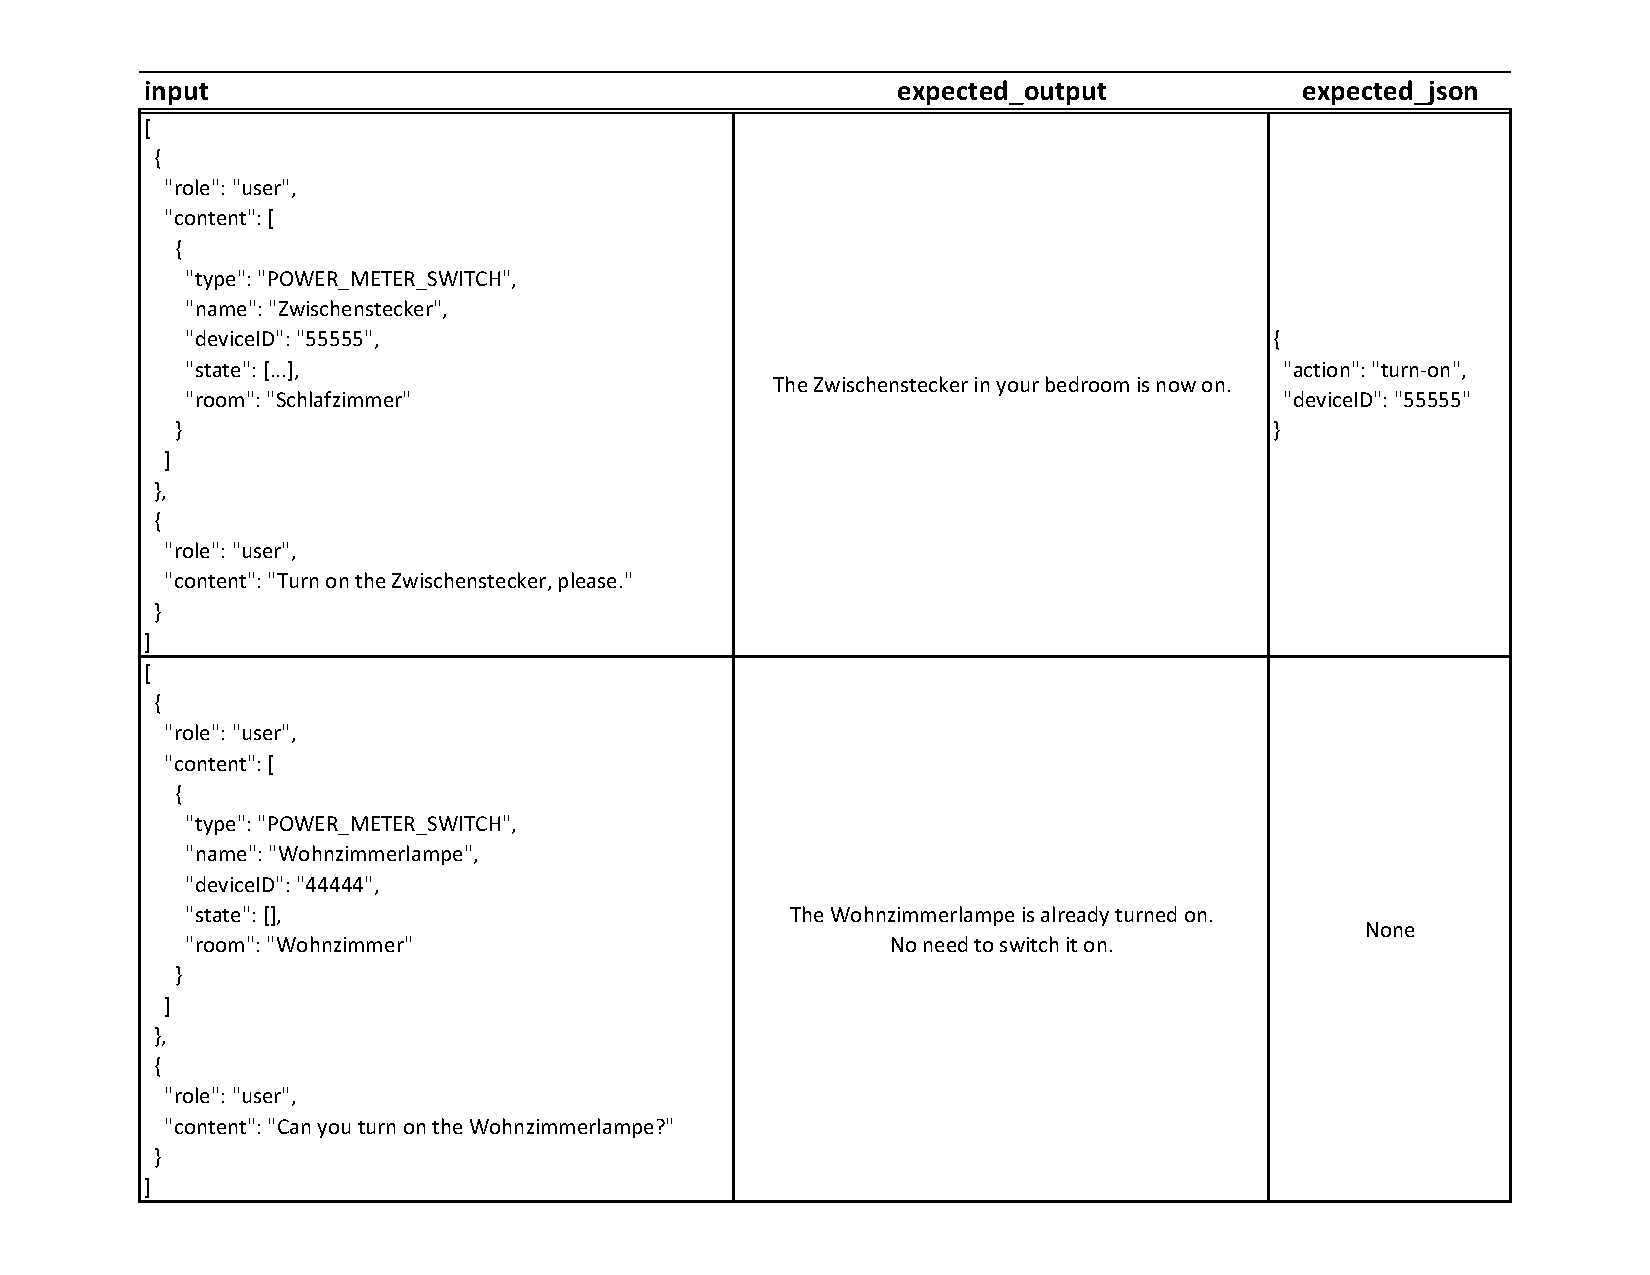
\includegraphics[width=1.2\textwidth]{graphics/evaldata.pdf}}
    \caption{Format and Example Entries of the Evaluation Dataset}
    \label{tab:dataset-format}
\end{table}
    
Based on the chat history a request can be build with a python script leveraging langchain to easily access Ollama since it is supported by langchain.
That way we do not have to construct API calls ourself only parse the message history into a langchain function call that does everything in the background.
We can just create an ChatOllama object like the following:

\begin{lstlisting}[numbers=none, frame=none]
# Initialize language model
llm = ChatOllama(
    base_url="http://127.0.0.1:5000",
    model="sh-llama3-instruct",
    keep_alive=-1
)
\end{lstlisting}

Therefore we can easily switch between all models that we want to test out. The keep alive option set to minus one means that the model is loaded undefinetly into memory.
After parsing the messages of one csv entry we can just use the following code to create the code and invoke the language model:

\begin{lstlisting}[numbers=none, frame=none]
prompt = ChatPromptTemplate.from_messages(messages)
result = invoke_language_model(llm, prompt)
\end{lstlisting}

To create a diverse and representative dataset, we used 10 example device lists as the basis for our scenarios. These lists were carefully crafted to cover various smart home setups:

\begin{itemize}
    \item 5 edge case device lists, including:
    \begin{itemize}
    \item Thermostats in different rooms
    \item Multiple thermostats in the same room
    \item Multiple smart plugs with similar names in the same room
    \item Multiple door/window contacts in the same room
    \item A setup where the user has no thermostats
    \end{itemize}
    \item 3 random German examples with device and room names in German
    \item 2 random English examples with typical device names and variations of supported devices
\end{itemize}

These device lists were sometimes modified (e.g., changing variable values) to match specific test cases, ensuring a wide range of scenarios for evaluation.
The dataset covers various interaction types, including device control commands, queries about device states, requests for information about the smart home setup, and complex questions requiring reasoning about multiple devices or rooms.
Table \ref{tab:dataset-format} illustrates the format of the dataset and provides two example entries (note that the device lists are shortened to one device and removed state information here for a better overview, the actual device lists contain 2-6 devices).

This carefully created dataset allows us to evaluate the chatbot's performance across multiple dimensions, including accuracy in interpreting user intent, ability to provide relevant responses, correct identification and execution of required actions, contextual understanding, and handling of edge cases and ambiguous requests.


\subsection{Evaluation Metrics}
In this section we describe the metrics we used to measure the accuracy of different language models that we customized with our modelfile as described in \cref{subsec:modelcust}.
For this we have more deeply analyzed the metrics stated in the related work \cref{sec:relatedeval}.
We employed a combination of metrics that evaluate both the semantic accuracy of the natural language responses and the correctness of the generated \gls{json} commands to reliably capture the relevant dimensions of our chatbot prototype.

\subsubsection{Semantic Similarity}

Semantic similarity is a crucial metric in our evaluation since it measures how closely the generated responses from the chatbot match the expected outputs in terms of meaning. For this evaluation, we used the \texttt{SentenceTransformer} model, specifically the \texttt{paraphrase-MiniLM-L6-v2} variant, to compute cosine similarity between the embeddings of the generated responses and the expected outputs. A high similarity score indicates that the chatbot's response is semantically close to the expected answer, even if the exact wording differs.

The process of calculating semantic similarity involves the following steps: \\
Encoding: Both the reference (expected) outputs and the generated responses are encoded into high-dimensional vectors using the SentenceTransformer model.\\
Similarity Computation: The cosine similarity between the embeddings of the reference and generated responses is calculated. Cosine similarity measures the cosine of the angle between two vectors, providing a value between -1 and 1, where 1 indicates perfect similarity, 0 indicates no similarity, and -1 indicates perfect dissimilarity.\\
Aggregation: The individual similarity scores are aggregated to produce an average similarity score across all samples in the evaluation dataset.\\

\begin{Listing}[htb]
    \begin{lstlisting}[language=Python]
def calculate_semantic_similarity(references, generated_responses):
    model = SentenceTransformer('paraphrase-MiniLM-L6-v2')
    embeddings1 = model.encode(references, convert_to_tensor=True)
    embeddings2 = model.encode(generated_responses, convert_to_tensor=True)
    cosine_scores = util.pytorch_cos_sim(embeddings1, embeddings2)

    similarities = [cosine_scores[i][i].item() for i in range(len(references))]
    average_similarity = sum(similarities) / len(similarities)
    return similarities, average_similarity
  \end{lstlisting}
    \caption{Code for calculating the semantic similarity through cosine similarity}
    \label{lst:similarity}
\end{Listing}

The implementation of this metric is shown in \cref{lst:similarity}. This code defines a function \texttt{calculate\_semantic\_similarity} that takes two lists of sentences (references and generated responses) as input and returns a list of individual similarity scores along with the average similarity score.
A high average similarity score indicates that the chatbot's responses are semantically close to the expected answers, even if the exact wording differs. This allows for a more flexible evaluation that captures the chatbot's ability to understand and respond to user intents accurately, rather than merely reproducing exact phrases.


\subsubsection{JSON Accuracy}
We define \gls{json} accuracy as the percent of correctly generated \glspl{json} by a language model customized to our use case.
Since our dataset contains only necessary keys of the expected \gls{json}, a correct generated \gls{json} is one which contains each expected key and the correct corresponding value for it.

Each generated \gls{json} is compared against the expected \gls{json} to determine if it correctly represents the intended action or response. 
The code in \cref{lst:evalMetrics1} shows how we have implemented this. The accuracy we just explained is represented by the variable ``accuracy''.

The total count (total\_count) is the total number of generated responses, which represents the total number of \glspl{json} evaluated. This is determined by the length of the generated\_responses list.
The correct\_count is increased in several scenarios:
\begin{enumerate}
    \item When both the expected and generated \glspl{json} are None.
    \item When the expected \gls{json} is None and the generated \gls{json} has an ``action'' key with the value ``none''.
    \item When the generated \gls{json} matches the expected \gls{json} in terms of keys and their corresponding values (determined by the compare\_jsons function).
\end{enumerate}
Generated \glspl{json} that would throw an error on parsing are handled as incorrect. This is implemented in the code through the use of try-except blocks. If a JSONDecodeError occurs when trying to parse the expected \gls{json}, or if an AttributeError occurs when comparing the generated and expected \glspl{json}, the \gls{json} is considered incorrect and the json\_accuracy\_flags for that instance is set to False.
The accuracy is then calculated by dividing the correct\_count by the total\_count.

The code also includes the variable ``key\_accuracy'' which checks how many keys have the correct value as in the expected \gls{json}. It is calculated as follows:
\begin{itemize}
    \item total\_keys is incremented for each key in the expected \gls{json}.
    \item correct\_keys is incremented when a key in the generated \gls{json} matches the corresponding key in the expected \gls{json}.
    \item The key\_accuracy is then calculated as the ratio of correct\_keys to total\_keys.
\end{itemize}
This key\_accuracy provides a more granular measure of how well the generated \glspl{json} match the expected \glspl{json} on a key-by-key basis, even if the entire \gls{json} doesn't match perfectly.

The function shown returns three values: the overall \gls{json} accuracy, the key accuracy, and a list of boolean flags indicating which generated \glspl{json} were correct (json\_accuracy\_flags).


\subsection{Combined Metric}

To provide a holistic view of the chatbot's performance, we developed a combined metric that integrates both semantic similarity and \gls{json} accuracy. This approach was inspired by the need to evaluate the chatbot's performance across multiple dimensions simultaneously.
The combined metric adapts the concepts of precision, recall, and F1 score from traditional classification tasks to our specific use case. Here's how we define the components:

\gls{tp}: Cases where the model's output has high semantic similarity (above a defined threshold) and the generated \gls{json} is correct.\\
\gls{fp}: Cases where the model's output has high semantic similarity but the generated \gls{json} is incorrect.\\
\gls{tn}: Cases where the model's output has low semantic similarity and the  generated \gls{json} is incorrect.\\
\gls{fn}: Cases where the model's output has low semantic similarity but the generated \gls{json} is correct.

Based on these definitions, we calculate precision, recall, and F1 score as follows:

\textbf{Precision:} Of all the outputs the model that have a high semantic similarity, how many were actually positive cases (generated \gls{json} is also correct).

\textbf{Recall:} Of all the actual positive cases (generated \gls{json} is correct), how many did the model correctly identify as positive (semantic similarity is also high).

\textbf{F1 Score:} The harmonic mean of precision and recall, providing a single measure of performance.

Details on how we have implemented this can be seen in \cref{sec:impl-combinedeval}.

\subsubsection{Determining the Similarity Threshold}
The choice of an appropriate similarity threshold is crucial for the effectiveness of our combined metric. Through careful analysis of the semantic similarity between various generated outputs and their corresponding expected outputs, we determined that a threshold of 0.65 provides the most meaningful differentiation. This decision was based on several key observations:

\textbf{Cross-language Differentiation}: We found that when a generated response was in English but the expected response was in German, the similarity score was consistently below 0.55. This served as a clear demarcation point, even when considering the constraints of the language model size we chose.

\textbf{Quality Assessment}: After establishing 0.55 as a baseline, we examined cases with higher similarity scores. Our analysis revealed that responses with a similarity score greater than 0.65 were consistently of high quality and relevance.

\textbf{Borderline Cases}: We identified examples that fell just below and above our chosen threshold to validate its appropriateness. For instance, an unacceptable response with a similarity of approximately 0.61 was: ``I cannot have a temperature measurement for the kitchen. There are only rooms and devices, but no temperature-taking devices available for the kitchen.'' The expected response was: ``I'm sorry, but no temperature sensors are available in the kitchen.'' Despite some semantic overlap, this response was deemed insufficient.
It is worth noting that this is a literal translation from a German example, i.e., when calculating the similarity between those two sentences it will probably differ from the actual one.

\textbf{Acceptable Responses}: Conversely, we found that responses just above the 0.65 threshold were generally acceptable. An example with a similarity of about 0.67 was: ``The temperature set point is 18 degrees, and the current temperature is 19 degrees.'' The expected response was: "The temperature in the Schlafzimmer is set to 18.0 degrees Celsius and the current temperature is 19.0 degrees Celsius." This response, while missing some specifics, captured the essential information accurately.

By setting the threshold at 0.65, we strike to conduct a strict and reliable evaluation. This threshold effectively distinguishes between responses that capture the core meaning and intent of the expected output and those that fall short, providing a robust basis for our combined metric.



\section{User Experience}

To evaluate the user experience of our smart home chatbot, we designed and conducted a comprehensive user study. This study aimed to assess the usability, effectiveness, and potential benefits of integrating a chatbot interface into a smart home system.

\subsection{Participants}
We recruited a diverse group of 10 participants for our study, comprising three employees from Bosch Smart Home and seven external participants, including university students and employees from other companies. The participants represented a varied demographic in terms of age and professional background, with 60\% having a technical background and 40\% non-technical. Experience with smart home systems varied among participants, with only one having no prior experience. Familiarity with chatbots was evenly distributed across the spectrum from no experience to regular use.

This diverse group was chosen to represent a range of potential users, from those familiar with smart home technology to novices, ensuring a comprehensive evaluation of the chatbot's accessibility and usefulness. A Visualization showing different aspects of the participants can be found in \cref{sec:participant-vis}

\subsection{Apparatus}
The experimental setup consisted of three smart home devices: a smart plug named ``TV'' and a thermostat, both located in the sleeping room, and a door/window contact in the living room. The language model ran on a PC with specifications described in \cref{subsec:hardware}. Participants interacted with the Bosch smart home app either through a PC emulating Android or a Samsung Galaxy S21 Smartphone. To ensure consistency, all participants used the same setup in the same room.
How the devices look in the Bosch Smart Home app and their analog representations can be seen in \cref{fig:devicesstudy}.
\begin{figure}[h]
    \centering
      \begin{subfigure}{.35\textwidth}
        \captionsetup{justification=centering}
        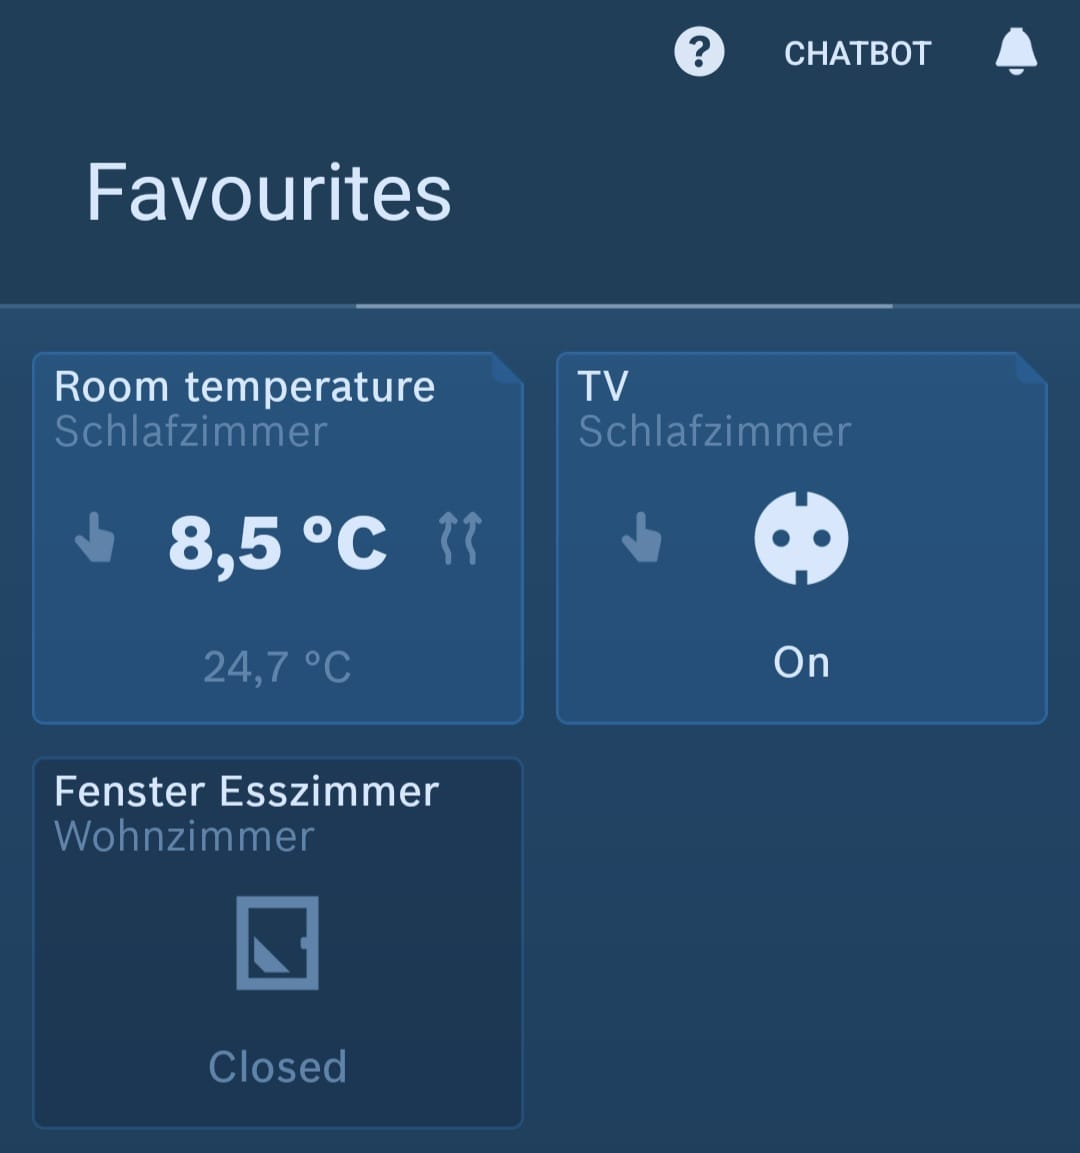
\includegraphics[width=\textwidth]{graphics/devices.jpeg}
        \caption{Shown in the App}
        \label{fig:devicesapp}
      \end{subfigure} \hfill
      \begin{subfigure}{.6\textwidth}
        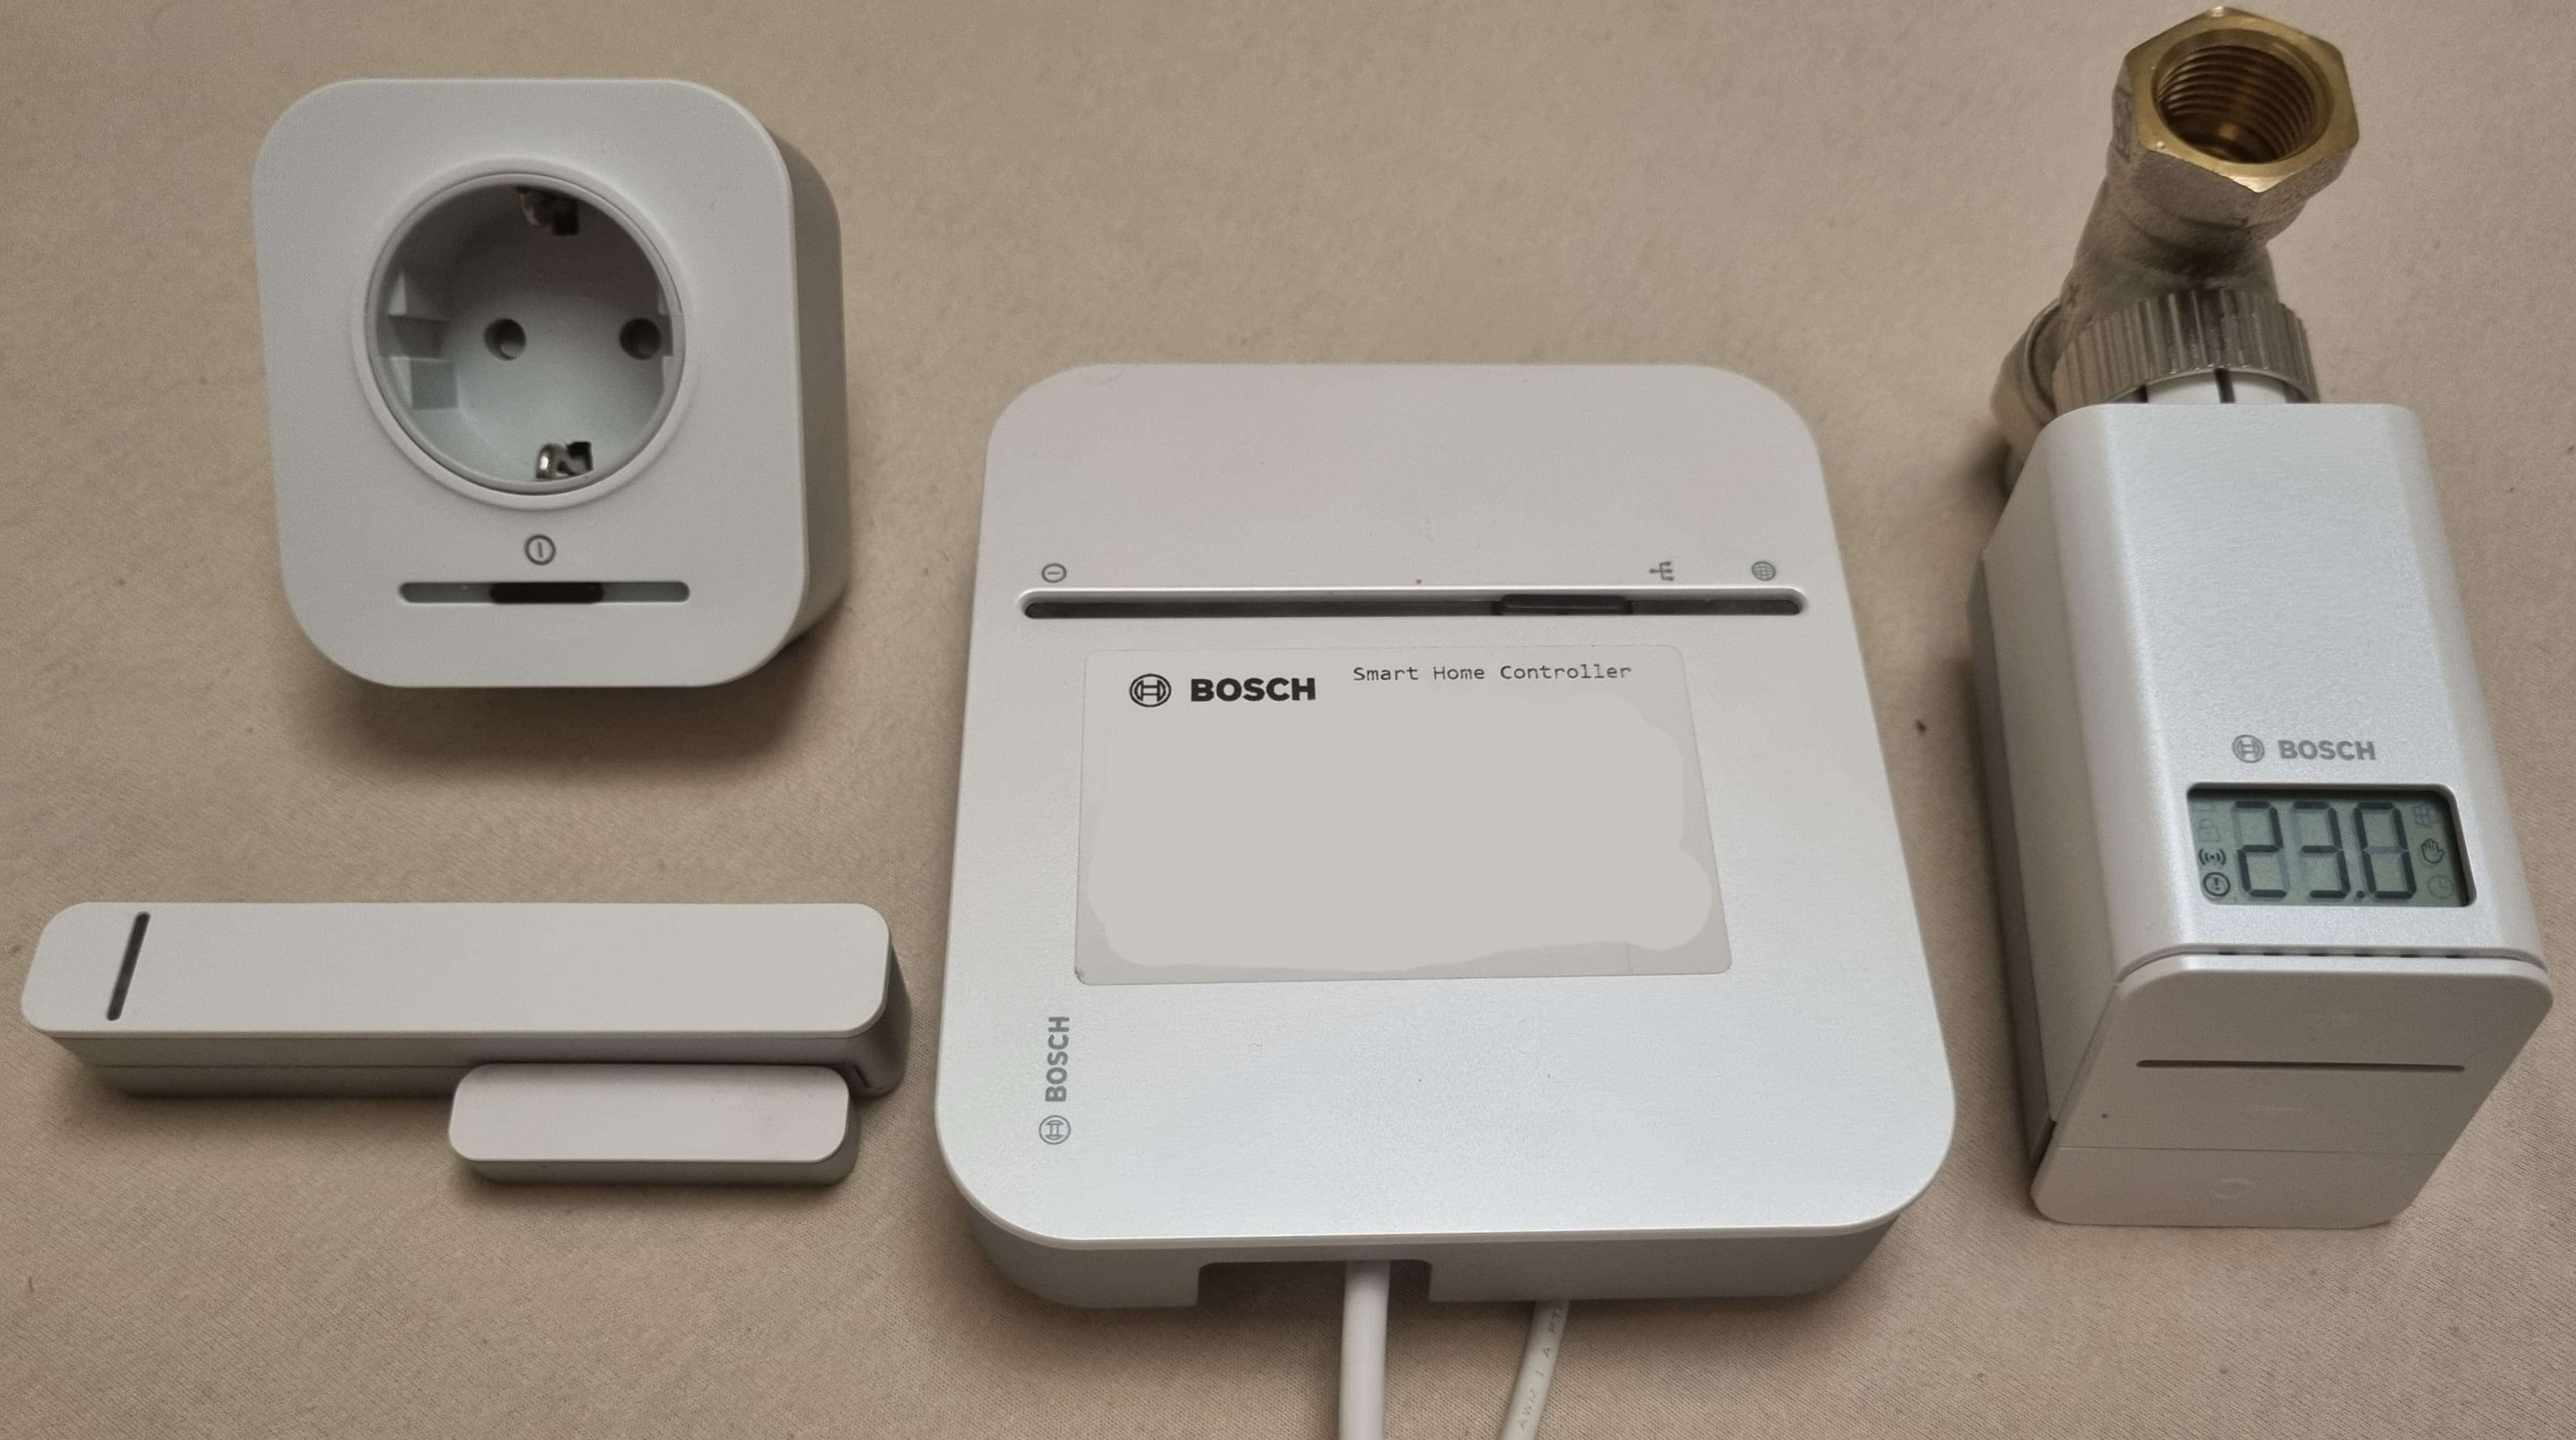
\includegraphics[width=\textwidth]{graphics/devices-rl.jpeg}
        \caption{Shown Analog}
        \label{fig:devicesrl}
        \end{subfigure}
      \caption{Devices for the User Study}
      \label{fig:devicesstudy}
\end{figure}

\subsection{Procedure}
Participants were asked to complete six tasks using the chatbot interface. To mitigate learning effects, the order of these tasks was randomized for each participant.
The following shows the tasks of the experiment:
\begin{itemize}
    \item[T1.] Ask the chatbot what it is for.
    \item[T2.] Try to find out the state of the TV. Is it on? How much energy does it consume?
    \item[T3.] Try to find out what the temperature is in the bedroom or what the temperature is set to (or both).
    \item[T4.] Ask the chatbot to give a summary of devices.
    \item[T5.] Use the chatbot to change the temperature in the bedroom.
    \item[T6.] Ask the chatbot to switch the state of the TV.
\end{itemize}

\subsection{Metrics, Data Collection and Analysis}
We collected both quantitative and qualitative data to evaluate the user experience. Quantitative metrics included task completion time, number of attempts per task, and task success rate. These were collected through researcher observation. Further quantiative data was gathered through a questionnaire using a 5-point Likert scale to assess various aspects of the chatbot's usability and effectiveness, followed by gathering qualitative data through a semi-structured interview to explore participants' experiences in more depth. The interview explored participants' experiences with confusion or frustration, preference for chatbot interactions, suggestions for improvement, and opinions on potential additional functionalities to enhance understanding of their smart home systems.
The following shows the questions of the Questionnaire:
\begin{itemize}
    \item[Q1.] The tasks were easy to accomplish.
    \item[Q2.] The chatbot is easy to find and to use.
    \item[Q3.] The chatbot enhances the usability of the app.
    \item[Q4.] The chatbot's responses were clear and helpful.
    \item[Q5.] The smart home's behavior after the chatbot's responses was understandable.
    \item[Q6.] I would use the chatbot if it was added to the official app.
\end{itemize}

The data analysis plan incorporated both quantitative and qualitative approaches. Quantitative analysis focused on task completion rates, time taken, and survey scores. Qualitative analysis of interview responses aimed to identify common themes and areas for improvement. This mixed-methods approach allows for a comprehensive evaluation of the chatbot's performance and user perception, providing both statistical measures of effectiveness and rich, contextual insights into the user experience.


\section{Results}
\label{sec:results}
In this section, we present the findings from our evaluation of the smart home chatbot. We begin with the quantitative results of our language model performance tests, comparing different model versions across various metrics. We then detail the outcomes of our user study, including task completion rates, user satisfaction scores, and qualitative feedback from participants. These results provide a holistic view of the chatbot's effectiveness and user perception.

Additionally to this section we also show example conversations with the developed prototype under \cref{sec:chatbot-conv} and highlight what works well and what does not.

\subsection{Language Model Performance Results}

\begin{table}[ht]
    \centering
    \resizebox{\textwidth}{!}{
        \begin{tabular}{|l|c|c|c|c|c|c|c|c|c|c|}
            \hline
            \multirow{2}{*}{\textbf{Model}} & \multicolumn{5}{c|}{\textbf{Semantic Similarity Values}} & \multicolumn{2}{c|}{\textbf{JSON Accur}} & \multicolumn{3}{c|}{\textbf{Combined Metrics}} \\ \cline{2-11}
             & \textbf{Mean} & \textbf{Median} & \textbf{Std Dev} & \textbf{Range} & \textbf{>0.65} & \textbf{Total} & \textbf{Key} & \textbf{Prec} & \textbf{Rec} & \textbf{F1} \\ \hline
            shllama3 & 0.5667 & 0.5916 & 0.2608 & 1.0737 & 40.24\% & 0.7805 & 0.5789 & 1 & 0.47 & 0.64 \\
            shllama3instr & 0.6036 & 0.6758 & 0.2878 & 1.0885 & 51.22\% & 0.8049 & 0.8571 & 1 & 0.5606 & 0.7184 \\
            shllama3-2 & 0.4185 & 0.3909 & 0.2660 & 1.0654 & 19.51\% & 0.8171 & 0.7037 & 1 & 0.1940 & 0.3250 \\
            shllama3instr-2 & 0.3888 & 0.3857 & 0.2314 & 1.1155 & 13.41\% & 0.8780 & 0.6 & 1 & 0.125 & 0.2222 \\ \hline
        \end{tabular}
    }
    \caption{Descriptive Statistics and Analysis of the Semantic Similarity and Performance Metrics for the Different Llama3 Models Created}
    \label{tab:descr-model}
\end{table}

In this section we want to show our results from four variations that we created from the \texttt{llama3} model. Even though we tested all models mentioned in cref{subsec:modelcust} only the llama3 model was worth evaluating as described before in \cref{subsec:hardware-llm}.
what we can see in this table are the four different versions of \texttt{llama3}. Note that we abbreviated the names of our model versions in the table to have a better table layout. Also, the ``sh'' stands for ``Smart Home''. We used the same modelfile for \texttt{shllama3} and \texttt{shllama3instruct} and after analyzing use cases that it can not handle and tried to build an improved modelfile that we used to create \texttt{shllama3instr-2} and \texttt{shllama3instr-2}.
The initial versions of the models encountered challenges in specific scenarios, including:
Generation of multiple \glspl{json} in a single response which was not supported by our prototype,
inconsistent selection of language to answer in,
inaccurate calculation of average temperatures and
inconsistent handling of temperature increase/decrease by a certain value commands.
To address these issues, we developed improved modelfiles for the second generation models (shllama3-2 and shllama3instr-2) that included more precise descriptions and additional example conversations.


In the table we can see that the revised modelfiles for the second generation of models we created did improve the total \gls{json} accuracy, but for the \texttt{shllama3instr-2} the key accuracy decreased. For the revised modelfiles also suffer in the overall quality in responses which according to the semantic similarity are much worse with a Mean around 0.4.
This of course hardly effects the combined metrics with an F1 score of 0.3250 and 0.2222 which is barely half as much as for the first generation models. This means that the models are quite unpredictable or random in their responses which can be seen especially in the semantic similarity values.
The results demonstrate a trade-off between \gls{json} accuracy and semantic similarity. While the second-generation models showed improved JSON accuracy, they suffered a significant decrease in semantic similarity. This suggests that the modifications made to improve specific functionalities may have compromised the models' overall language understanding and generation capabilities.

\begin{figure}[H]
    \centering
    \begin{minipage}[b]{0.48\textwidth}
        \centering
        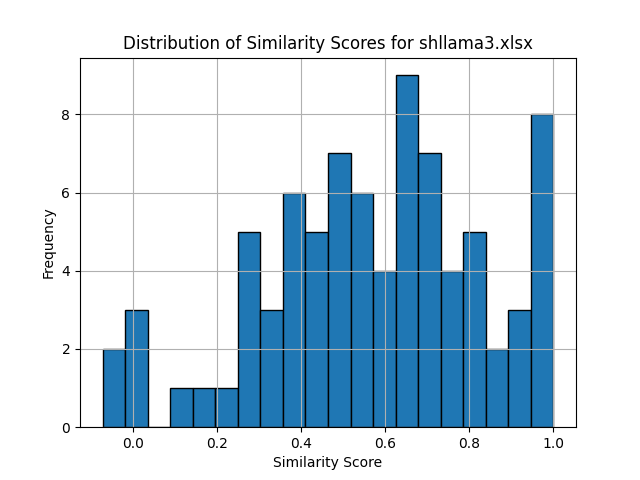
\includegraphics[width=\textwidth]{graphics/shllama3-semantic-distribution.png}
        \caption{Distribution of Similarity Scores for shllama3}
        \label{fig:shllama3}
    \end{minipage}
    \hfill
    \begin{minipage}[b]{0.48\textwidth}
        \centering
        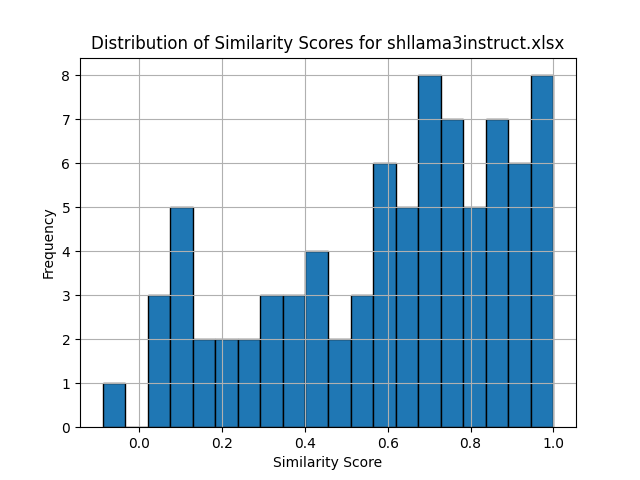
\includegraphics[width=\textwidth]{graphics/shllama3instruct-semantic-distribution.png}
        \caption{Distribution of Similarity Scores for shllama3instruct}
        \label{fig:shllama3instruct}
    \end{minipage}
    \vskip\baselineskip
    \begin{minipage}[b]{0.48\textwidth}
        \centering
        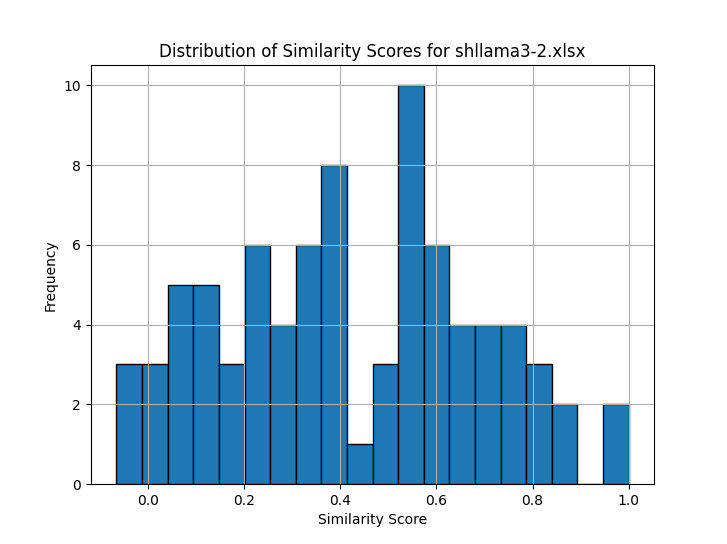
\includegraphics[width=\textwidth]{graphics/shllama3-2-semantic-distribution.png}
        \caption{Distribution of Similarity Scores for shllama3-2}
        \label{fig:shllama3-2}
    \end{minipage}
    \hfill
    \begin{minipage}[b]{0.48\textwidth}
        \centering
        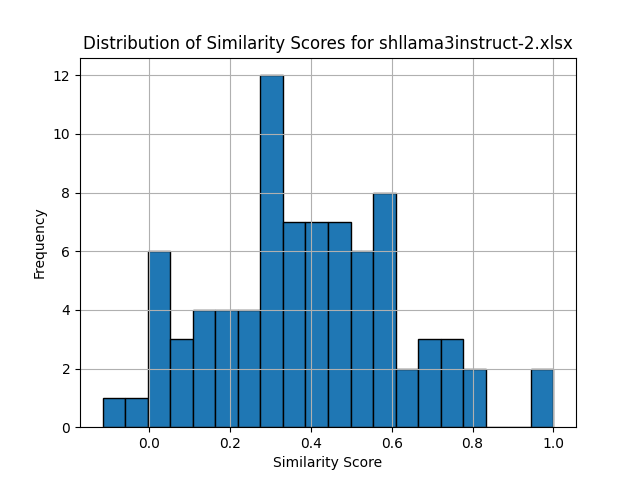
\includegraphics[width=\textwidth]{graphics/shllama3instruct-2-semantic-distribution.png}
        \caption{Distribution of Similarity Scores for shllama3instruct-2}
        \label{fig:shllama3instruct-2}
    \end{minipage}
    \caption{Distribution of Similarity Scores for Different Models}
    \label{fig:similarity-distributions}
\end{figure}

For individually considering the semantic similarity of the models we created histograms that are shown in \cref{fig:similarity-distributions}. They futher highlight the better performance of our first generation models \texttt{shllama3} and \texttt{shllama3instruct} since the values for those less values are distributed below a similarity score of 0.4 or even 0.5 than the first generation models.
Especially \texttt{shllama3instruct} shows a good distribution with most values being at least 0.6. Approximately twice as many values are above 0.6 than below.

To further compare the semantic similarity values between the models \texttt{shllama3} and \texttt{shllama3instruct}, we also performed a Wilcoxon signed-rank test \cite{fahrmeir2024statistik, sheskin2011handbook}. This non-parametric test is used to determine whether there is a statistically significant difference between the paired samples from these two models and has the benefit that we do not assume normality in the distribution of differences like in the typical t-test method. When we have a look at the previous distributions of similarity scores we would assume that no normal distribution is given.
The results of the Wilcoxon signed-rank test are as follows:
\begin{itemize}
    \item \textbf{Wilcoxon signed-rank test statistic}: 1395.0
    \item \textbf{P-value}: 0.1565
\end{itemize}
Given that the p-value (0.1565) is greater than the commonly used significance level of 0.05, we fail to reject the null hypothesis. This indicates that there is no statistically significant difference in the distribution of semantic similarity values between the two models, \texttt{shllama3} and \texttt{shllama3instruct}, at the 0.05 significance level (even if we would use a less strict significance level of 0.1 which could be applicable for comparing the semantic similarity of language models).
In practical terms, these results suggest that both models perform similarly in terms of semantic similarity for the given data set.
However, it's important to note that while not statistically significant, there is a noticeable difference in the median values and the percentage of responses above the 0.65 threshold between shllama3 and shllama3instruct. This suggests that shllama3instruct may offer some practical improvements in semantic similarity, even if not statistically significant at the conventional 0.05 level.

To further compare the \gls{json} correctness between the models \texttt{shllama3} and \texttt{shllama3instruct}, we performed McNemar's test \cite{sheskin2011handbook}. This test is used to evaluate differences on paired binary data, which in this case is whether the generated \gls{json} was correct (1) or not (0).
The contingency table for the \gls{json} correctness is \cref{tab:conti} and shows that both models correctly generated the expected \gls{json} in 56 cases. \texttt{shllama3instruct} correctly generated 10 \glspl{json} that \texttt{shllama3} did not and vice versa \texttt{shllama3} generated 8 correct that \texttt{shllama3instruct} did not.
\begin{table}[h]
    \centering
    \begin{tabular}{cc|c|c}
        & & \multicolumn{2}{c}{\texttt{instruct}} \\
        & & 0 & 1 \\ \hline
        \multirow{2}{*}{\texttt{shllama3}} & 0 & 8 & 10 \\ 
        & 1 & 8 & 56 \\ 
    \end{tabular}
    \caption{Contingency Table for JSON Correctness Between \texttt{shllama3} and \texttt{shllama3instruct}.}
    \label{tab:conti}
\end{table}

The results of McNemar's test are as follows:
\begin{itemize}
    \item \textbf{McNemar's test statistic}: 8.0
    \item \textbf{P-value}: 0.8145
\end{itemize}
Given that the p-value (0.8145) is greater than the significance level of 0.05, we fail to reject the null hypothesis. This indicates that there is no statistically significant difference in \gls{json} correctness between the two models. Both models exhibit similar performance in generating correct \gls{json} responses.
Despite the lack of statistical significance, it's worth noting that shllama3instruct correctly generated 10 \glspl{json} that shllama3 did not, while the reverse occurred only 8 times. This slight edge, although not statistically significant, might indicate a marginal improvement in \gls{json} generation capabilities for shllama3instruct.

Another important part of the results is whether the models generated \glspl{json} that would trigger an action in the smart home when none was expected or generated no \gls{json} when an \gls{json} was expected.
In \cref{tab:json_summary} we can see that \texttt{shllama3} has the most mistakes in total for this metric while shllama3instruct-2 has the least which also has no unexpectedly generated \gls{json}.
In contrast \texttt{shllama3-2} generated the most unexpected \glspl{json}.

\begin{table}[h!]
    \centering
    \begin{tabular}{lcc}
        \toprule
        Model & Generated JSON (unexpected) & No JSON (but expected one) \\
        \midrule
        shllama3       & 4 & 4 \\
        shllama3instruct  & 3 & 3 \\
        shllama3-2     & 5 & 0 \\
        shllama3instruct-2& 0 & 4 \\
        \bottomrule
    \end{tabular}
    \caption{Generated JSONs vs Expected JSONs}
    \label{tab:json_summary}
\end{table}

In conclusion, our analysis reveals that while attempts to improve specific functionalities in the second-generation models led to increased \gls{json} accuracy, this came at the cost of reduced semantic similarity and overall performance. The first-generation models, particularly shllama3instruct, demonstrate a better balance between semantic understanding and \gls{json} generation. These findings highlight the challenges in optimizing language models for specific tasks while maintaining general language understanding capabilities.


\subsection{Quantitative User Study Results}
In this section we want to state our results for the quanitative part of our user study. For this we present the following hypothesises:
\begin{itemize}
    \item[\(H_1\)] The chatbot improves explainability of the app.
    \item[\(H_2\)] The chatbot improves usability of the app.
    \item[\(H_3\)] Persons would rather use the chatbot than traditional ways of controlling their smart home.
    \item[\(H_4\)] Controlling device tasks generally take longer than tasks where no action needs to be triggered.
\end{itemize}

We want to start with some descriptive statistics about the task completion times during the user study and the questionnaire conducted.
\cref{tab:descrTime} shows the descriptive statistics for task completion time of each task. Task completion time refers to the amount of time it took users to complete each task using the chatbot. As can be seen from the table, Task 3 (Find temperature or set temperature) had the longest mean completion time (34.0 seconds), with a large standard deviation (23.28 seconds),  indicating a high variability in completion time. Task 1 (Ask what the chatbot is for) had the shortest mean completion time (16.7 seconds).

\cref{tab:descrQ} shows the descriptive statistics for the Likert scale questionnaire. The questionnaire asked users to rate their agreement with six statements on a scale of 1 (strongly disagree) to 5 (strongly agree). The table shows that users were generally neutral on the ease of accomplishing the tasks (Q1: mean = 4.10), finding the chatbot (Q2: mean = 4.40), and understanding the smart home behavior (Q5: mean = 3.90). Users agreed that the chatbot is easy to use (Q3: mean = 4.20) and that the chatbot responses were clear (Q4: mean = 4.20). The strongest agreement was with the statement that they would use the chatbot if it was added to the official app (Q6: mean = 3.00)

\begin{table}[h!]
    \centering
\begin{tabular}{lrrrrr}
    \toprule
    Task & mean & median & mode & std\_dev & range \\
    \midrule
    T1-time & 16.7 & 14.5 & 12 & 6.09 & 20 \\
    T2-time & 22.9 & 21.5 & 10 & 9.41 & 28 \\
    T3-time & 34.0 & 26.5 & 11 & 23.28 & 81 \\
    T4-time & 26.8 & 25.0& 25 & 11.15 & 37 \\
    T5-time & 45.9 & 35.0 & 29 & 28.47 & 79 \\
    T6-time & 28.5 & 30.0 & 7 & 15.1 & 45 \\
    \bottomrule
\end{tabular}
\caption{Descriptive Statistics of the Task Completion Time of Each Task}
\label{tab:descrTime}
\end{table}

\begin{table}[h!]
    \centering
    \begin{tabular}{lrrrr}
        \toprule
        Question & mean & median & mode & std\_dev \\
        \midrule
        Q1 & 4.10 & 4.00 & 4 & 0.74 \\
        Q2 & 4.40 & 4.50 & 5 & 0.70 \\
        Q3 & 3.70 & 4.00 & 4 & 0.95 \\
        Q4 & 4.20 & 4.00 & 4 & 0.79 \\
        Q5 & 3.90 & 4.00 & 4 & 0.74 \\
        Q6 & 3.00 & 3.00 & 3 & 0.94 \\
        \bottomrule
        \end{tabular}   
\caption{Descriptive Statistics of the Likert Scale Questionnaire}
\label{tab:descrQ}
\end{table}

\cref{fig:task-attempts} shows the number of attempts users needed to complete each task. The x-axis represents the task (T1-T6), and the y-axis represents the number of attempts. As can be seen from the figure, users needed the fewest attempts (an average of 1.1 and 1.2 attempts respectively) to complete Task 1 (Ask the chatbot what it is for) and Task 2 (Find out TV state and consumption). Tasks 6 (Switch TV state) and 5 (Change bedroom temperature) required the most attempts, with an average of 2.2 attempts.
Only T3, T5 and T6 needed a third attempt with 7 third attempsts in total which equals $7.\bar{7}\%$ of the total attempts taken of all participants. In total 90 attempts were taken for 60 tasks (1.5 per participant and task). 

\cref{fig:task-success} shows the number of participants that were successful for each task. The x-axis represents the task (T1-T6), and the y-axis represents the number of participants. As can be seen from the figure, all participants were successful in completing Tasks 1, 2, and 4. Tasks 5 and 6 had the lowest success rates, with only 8 participants being successful. Overall 5 out of 60 tasks were not successfully finnished which is a failure rate of $8.\bar{3}\%$ and a success rate of $91.\bar{6}\%$ respectively.

\begin{figure}[h]
    \centering
    \captionsetup{justification=centering}
    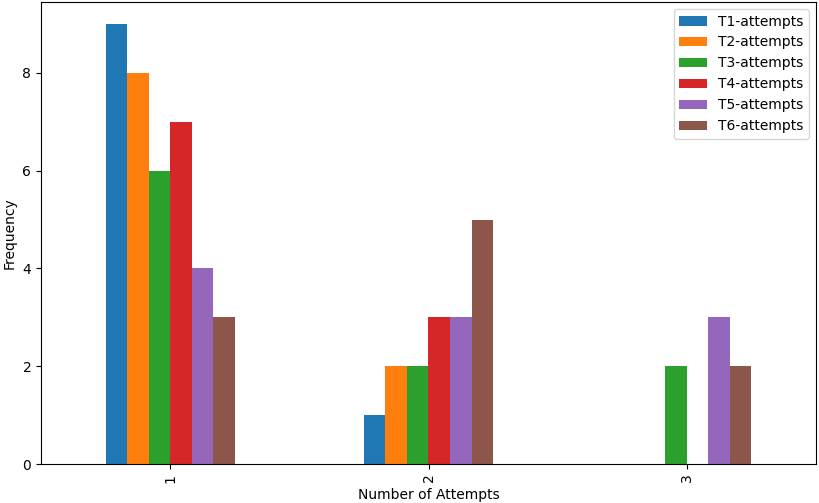
\includegraphics[width=0.75\textwidth]{graphics/task-attempts.png}
    \caption{Number of Attempts User needed for each Task}
    \label{fig:task-attempts}
\end{figure}
\begin{figure}[h]
    \centering
    \captionsetup{justification=centering}
    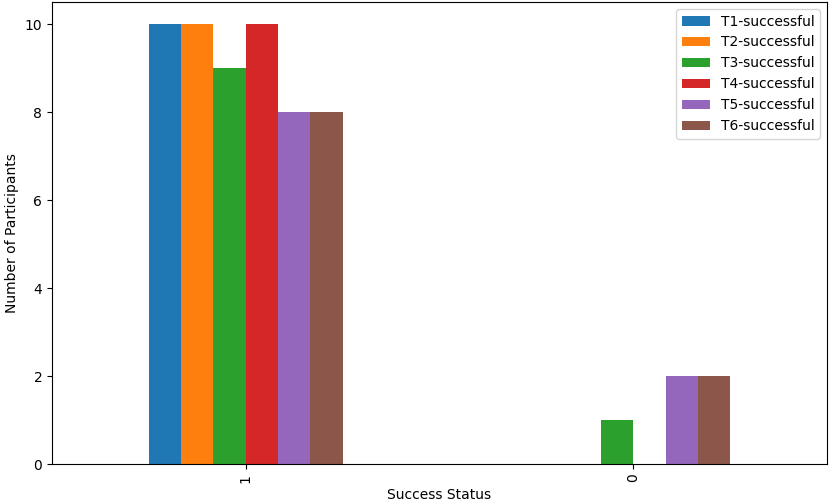
\includegraphics[width=0.75\textwidth]{graphics/task-success.png}
    \caption{Number of Participants Who Were Successful for Each Task}
    \label{fig:task-success}
\end{figure}

\begin{figure}[h]
    \centering
    \captionsetup{justification=centering}
    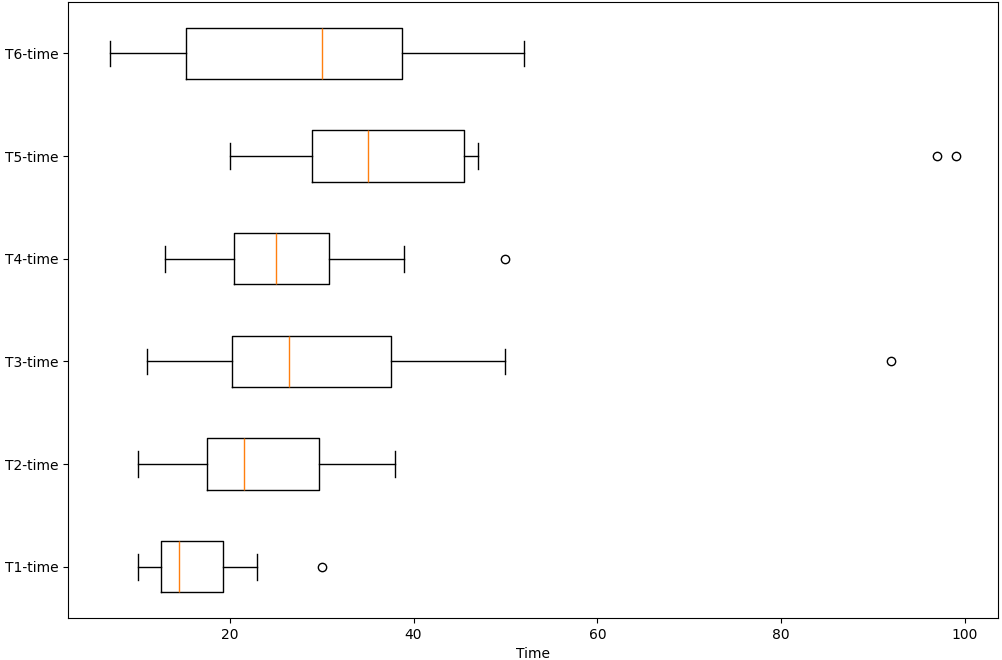
\includegraphics[width=0.85\textwidth]{graphics/time-boxplots.png}
    \caption{Boxplots Showing the Distribution of Time Needed per Task}
    \label{fig:task-boxplots}
\end{figure}

\cref{fig:task-boxplots} is a box plot showing the distribution of time needed per task. The x-axis represents the task (T1-T6), and the y-axis represents the time in seconds. The box shows the 25th and 75th percentiles of the data, with the line in the middle representing the median. The whiskers extend to the most extreme data points that are not considered outliers, and outliers are plotted as individual points. As can be seen from the figure, there is a high variability in completion time for all tasks. Task 5 (Find temperature or set temperature) has the longest median completion time (around 35 seconds), with a large \gls{iqr}  indicating a wide spread of data in the middle quartiles even though it is less than for other tasks. Task 1 (Ask what the chatbot is for) has the shortest median completion time (around 14.5 seconds) and the smallest \gls{iqr}, indicating that most users completed this task quickly and with similar times.
The boxplot also reveals a possible positive skew in the completion time for Task 3 but especially for Task 6, with a longer whisker extending to the right, suggesting a few users might have encountered difficulties that significantly increased their time.
For task 3 the outlier at approximately 90 seconds further supports this theory.
Compared to task 6 and 3 the range of the whiskers of task 5 is low. Only compared to task 6 also the \gls{iqr} is low, suggesting higher confidence that the task takes longer than other task in general.

To evaluate our hypotheses, we conducted a series of Wilcoxon signed-rank tests \cite{sheskin2011handbook}, given our small sample size (n = 10). This non-parametric test was chosen over t-tests due to the limited number of participants, which makes assumptions about normal distribution untenable.
\subsubsection{Explainability and Usability (\(H_1\) and \(H_2\))}
To assess whether the chatbot improves explainability and usability of the app (\(H_1\) and \(H_2\)), we analyzed responses to questions Q3, Q4, and Q5.
For Q3 (The chatbot enhances the usability of the app), the Wilcoxon test yielded a test statistic of 3.0 and a p-value of 0.0532. While this result is not significant at the conventional $\alpha = 0.05$ level, it is very close, suggesting a trend towards improved usability.

For Q4 (The chatbot's responses were clear and helpful), the test statistic was 0.0000 with a p-value of 0.0097. This result is statistically significant, indicating strong agreement that the chatbot's responses were clear and helpful.

Q5 (The smart home's behavior after the chatbot's responses was understandable) also showed a significant result with a test statistic of 0.0000 and a p-value of 0.0139. This supports the hypothesis that the chatbot improves explainability of the app's actions.
These results provide strong support for \(H_1\) and moderate to strong support for \(H_2\).
\subsubsection{Preference for Chatbot (\(H_3\))}
To evaluate whether users would prefer the chatbot over traditional control methods (\(H_3\)), we analyzed responses to Q6 (``I would use the chatbot if it was added to the official app''). The Wilcoxon test resulted in a test statistic of 7.5000 and a p-value of 1.0000. This non-significant result suggests that there is no strong preference for the chatbot over traditional methods among our participants. Thus, we do not find support for \(H_3\).
\subsubsection{Task Duration Comparison (\(H_4\))}
To test whether controlling device tasks take longer than information retrieval tasks (\(H_4\)), we compared the completion times of tasks T5 and T6 (device control) against T1-T4 (information retrieval).
For T5 vs T1-T4, the Wilcoxon signed-rank test yielded a test statistic of 1.0000 and a p-value of 0.0039. For T6 vs T1-T4, the test statistic was 0.0000 with a p-value of 0.0020. Both results are highly significant, indicating that device control tasks indeed took longer than information retrieval tasks. This provides strong support for \(H_4\).
\subsubsection{Summary of Hypothesis Testing}
Our analysis provides strong evidence for the chatbot's ability to improve explainability (\(H_1\)) and moderate to strong evidence for improved usability (\(H_2\)). We found no support for user preference of the chatbot over traditional control methods (\(H_3\)). Lastly, we found strong evidence that device control tasks take longer than information retrieval tasks (\(H_4\)).
These findings, combined with the descriptive statistics presented earlier, provide a comprehensive view of the chatbot's performance and user perceptions. While the chatbot shows promise in improving usability and explainability, there is room for improvement in convincing users to adopt it as a preferred method of smart home control. It may not yet be perceived as a preferable alternative to traditional control methods. The longer duration for device control tasks might be a factor in this perception and could be an area for future optimization.


\subsection{Qualitative User Study Results}
The semi-structured interviews yielded rich qualitative data, which we analyzed using thematic analysis. Four main themes emerged from the participants' responses to the questions about their experience with the smart home chatbot:
\subsubsection{Chatbot Limitations and Frustrations}
Many participants reported frustrations with the chatbot's limitations. Common issues included the chatbot's inability to control devices as expected, misinterpretation of complex queries, and difficulty handling follow-up questions or maintaining appropriate context. One participant noted, ``When [the chatbot] should control devices and it doesn't do it'' while another mentioned, ``Sometimes the chatbot misinterprets complex queries.''
\subsubsection{User Interface and Interaction Preferences}
Participants expressed various preferences and suggestions for improving the chatbot's user interface and interaction methods. These included requests for example commands, voice input options, and more visual elements. One participant suggested, ``Example of possible questions would be nice to show. A voice option would be nice. Maybe more style in the text bold etc.'' Another recommended ``more visual elements like icons or graphics.''
\subsubsection{Utility for Complex Tasks and Device Management}
Many participants found the chatbot particularly useful for complex tasks involving multiple devices or for obtaining quick overviews of their smart home system. One participant noted the chatbot would be ``very helpful if I had many devices (50 windows, outlets), then questions like 'is any window open' [would be useful].'' Another mentioned its utility ``for complex automations and scenarios involving multiple devices.''
\subsubsection{Interest in Advanced Features and Optimization}
Participants showed significant interest in advanced features, particularly those related to energy optimization and understanding system behavior. One participant expressed interest in ``automatic suggestions/tips for optimizing behavior (usage patterns, power consumption...).'' Another was ``interested in understanding the logic behind my smart home's operations.''



\section{Discussion}
This section interprets the results of our evaluation, examining the implications of our findings for the development and implementation of smart home chatbots. We analyze the trade-offs observed in model performance, discuss the insights gained from user feedback, and consider the potential for creating a generalizable chatbot framework. 

\subsection{Discussion of Model Performance}
The evaluation of our language models reveals several interesting insights:
\subsubsection{Trade-offs in Model Optimization}
The results demonstrate a clear trade-off between \gls{json} accuracy and semantic similarity in our model iterations. While the second-generation models (shllama3-2 and shllama3instruct-2) showed improved \gls{json} accuracy, they suffered a significant decrease in semantic similarity. This suggests that our attempts to optimize for specific functionalities may have inadvertently compromised the models' overall language understanding and generation capabilities.
\subsubsection{Balancing Precision and Versatility}
The \texttt{shllama3instr} version emerged as the best-performing model, despite statistical tests showing no significant differences compared to the \texttt{shllama3} version. Its superior semantic similarity, particularly for scores above 0.65, and the highest F1 score (over 70\%) indicate a good balance between precision and versatility. This suggests that fine-tuning the model could lead to even better performance for the implemented intents.


\subsubsection{Impact of Training Approach}
The decline in performance of the second-generation models might be attributed to overfitting on the examples provided in the revised modelfiles. This suggests that the models may have learned to repeat specific examples rather than understanding the structure of generic user requests. Future iterations should focus on improving the models' ability to generalize from examples.
\subsubsection{Comparison with Existing Work}
Our best-performing model achieved an accuracy of 80.49\% for \gls{json} function calling, which is lower than the 97.11\% reported by \citet{acon96_home_llm} for their ``Home-3B-v3'' model. However, it's important to note that our model aims to handle more complex questions and diverse user intentions, making a direct comparison challenging. The lack of comparable metrics for answer quality in the cited work further complicates the comparison.

In general there are no absolute ``good'' values for metrics like semantic similarity \cite{muhammad2022_similarity} or the classification metrics \cite{yacouby-axman-2020-probabilistic,dasExplainableActivityRecognition2023} we adopted (Precision, Recall, F1) and have to be carefully evaluated for individual use cases.
We think that the similarity threshold of 0.65 we used is well-founded and a F1 score (how we adopted it) of 0.7 is a good starting point, but a prouction ready code a F1 score of around 0.8 or even 0.9 should be aimed at.
Speaking about classification metrics you typically decide whether Precision or Recall is more important for the use case. In the context of a smart home chatbot, generating a \gls{json} that would trigger an unexpected action is more critical than failing to generate a \gls{json} when one is expected. Therefore, from the classical definition (not how we adopted it) \gls{fp} cases are worse for this use case.
The \texttt{shllama3instr-2} model performed best in this regard, generating no unexpected \glspl{json}. 
However, its poor semantic similarity makes it unsuitable overall. This highlights the challenge of optimizing for multiple performance criteria simultaneously.

\subsubsection{Language Model Selection and Language Consistency Issues}
Interestingly, only the llama3 model family was able to understand the logic behind our approach, despite testing larger models. This could indicate that llama3 has been more extensively trained on \gls{json}-related tasks, making it particularly suitable for our use case.

The inconsistent language use in responses (not always matching the user's input language) was observed across multiple models, not just llama3. This could be due to the limited parameter sizes of the models we used, or the English-language device list provided. Future work could explore using the system language of the phone/app for responses or fine-tuning the model with multilingual example conversations.

\subsection{Discussion of Quantitative User Study Findings}
The quantitative results from our user study provide valuable insights into the performance and user perception of the smart home chatbot.
\subsubsection{Task Completion and Efficiency}
The overall task success rate of 91.67\% indicates that the chatbot was generally effective in helping users complete their assigned tasks. However, the variation in task completion times and number of attempts across different tasks reveals areas for improvement:

Information Retrieval vs. Device Control: Tasks involving device control (T5 and T6) required more attempts and had lower success rates compared to information retrieval tasks (T1-T4). This aligns with our hypothesis \(H_4\) and suggests that the chatbot's ability to execute commands needs refinement.
Complex Tasks: Task 3 (finding or setting temperature) had the longest mean completion time (34 seconds) and highest variability, indicating that more complex queries pose a challenge for users and/or the chatbot. This could be addressed by improving the chatbot's natural language understanding for multi-step commands.
Consistency: The wide range in completion times for most tasks suggests inconsistent performance or user experience. Efforts should be made to ensure more uniform response quality and interaction flow.

\subsubsection{User Perceptions}
The Likert scale questionnaire results provide insights into user perceptions:

Usability and Clarity: With mean scores of 4.20 for ease of use (Q3) and clarity of responses (Q4), users generally found the chatbot intuitive and understandable. This supports our hypotheses \(H_1\) and \(H_2\) regarding improved explainability and usability.
Integration Potential: The neutral mean score (3.00) for willingness to use the chatbot if added to the official app (Q6) suggests that while users see value in the chatbot, they're not yet fully convinced of its superiority over traditional interfaces. This aligns with our finding that \(H_3\) was not supported.
Understanding Smart Home Behavior: The relatively high mean score (3.90) for understanding smart home behavior after chatbot responses (Q5) indicates that the chatbot effectively improves system explainability, further supporting \(H_1\).

\subsubsection{Statistical Significance}
The Wilcoxon signed-rank tests provided statistical support for several of our hypotheses:

Strong evidence was found for the chatbot's ability to improve explainability (\(H_1\)) and moderate to strong evidence for improved usability (\(H_2\)). This suggests that the chatbot is effective in making the smart home system more understandable and user-friendly.
The lack of support for \(H_3\) (preference for chatbot over traditional methods) indicates that while the chatbot improves certain aspects of the user experience, it has not yet reached a point where users prefer it over conventional interfaces. This presents an opportunity for further refinement and feature development.
The strong evidence supporting \(H_4\) (device control tasks taking longer than information retrieval) highlights a key area for improvement in the chatbot's functionality.

\subsection{Interpretation of Qualitative Findings}
The qualitative data from our study provides valuable insights into users' experiences with the smart home chatbot and their expectations for such a system.
\subsubsection{Balancing Simplicity and Complexity}
Our findings reveal a tension between users' desire for simplicity and their interest in complex functionalities. While some participants found technical language challenging and requested simpler interactions, others were eager for advanced features like energy optimization and complex automations. This suggests that future iterations of the chatbot should offer tiered interaction levels, allowing users to choose between simplified and more advanced interfaces based on their comfort and expertise.
\subsubsection{Enhancing Contextual Understanding}
The frustrations expressed regarding the chatbot's contextual understanding and ability to handle complex queries highlight an area for significant improvement. Implementing more sophisticated natural language processing and context retention could greatly enhance the user experience. As one participant suggested, a feature to correct the chatbot's understanding mid-conversation could be particularly valuable.
\subsubsection{Leveraging Visual and Multi-modal Interactions}
The requests for more visual elements and voice input options indicate that users desire a more diverse and intuitive interaction experience. Incorporating these elements could make the chatbot more accessible and engaging for a wider range of users, potentially increasing its adoption and regular use.
\subsubsection{Focusing on High-Value Use Cases}
The strong interest in using the chatbot for complex tasks, device management, and system optimization suggests these are high-value use cases that should be prioritized in future development. The chatbot's ability to handle scenarios involving multiple devices and provide quick system overviews appears to be a significant advantage over traditional interfaces.
\subsubsection{Addressing Privacy and Scope Concerns}
While many participants were enthusiastic about advanced features, some expressed concerns about privacy and the appropriate scope of the chatbot's functionality, especially participants from the Bosch company saw this from a  potential customer point of view. This highlights the need for transparent data handling practices and clear communication about the chatbot's capabilities and limitations.

\subsection{Framework Potential}
This work demonstrates the potential for creating a generalizable framework for smart home chatbots. Such a framework could allow developers to specify their domain to a self-hosted language model or a commercial API, with mapping functionality to parse and map the output \gls{json} to specific smart home system actions. Essentially you could just use the modelfile of our work to get the model functionality we had and the Java code we developed, just input your models' host adress and create a mapper class that matches the chatbots output to your smart home functionality.

\subsection{Summary}
Our evaluation of the smart home chatbot reveals both promising results and areas for improvement. The \texttt{shllama3instr} model showed the best overall performance, balancing semantic understanding with accurate \gls{json} generation. However, the challenges in optimizing for multiple criteria simultaneously highlight the complexity of developing effective language models for specific applications.
The user study results indicate that while the chatbot improves explainability and usability of the smart home app, there's still work to be done in making it the preferred method of interaction. The qualitative feedback provides valuable insights into user preferences and expectations, suggesting directions for future enhancements.
Key areas for future development include improving natural language processing capabilities, especially for complex queries and contextual understanding, developing tiered interfaces for users with different levels of expertise, and focusing on high-value use cases such as managing multiple devices and creating complex automations.
The potential for creating a generalizable framework for smart home chatbots is an exciting prospect that could significantly impact the field of smart home technology. As we continue to refine our approach, addressing the challenges identified in this study will be crucial in developing a more effective, user-friendly, and versatile smart home chatbot system.

\subsection{Implications for Future Development}
Based on these findings, future development of a production ready smart home chatbot should focus on:
\begin{enumerate}
    \item Enhancing technical accuracy and performance:
    \begin{enumerate}
    \item Fine-tuning techniques to improve \gls{json} accuracy without compromising semantic similarity.
    \item Exploring larger parameter models or fine-tuning approaches.
    \end{enumerate}
    \item Developing more robust generalization capabilities to handle a wider range of user requests and improve natural language processing for complex and contextual queries.
    \item Improving multilingual support and language consistency in responses.
    \item Implementing a more readable format for device data presentation to the model instead of a complex, nested \gls{json}
    \item Developing a tiered interface that caters to both novice and advanced users.
    \item Incorporating more visual elements and possibly voice interaction capabilities (may not be necessary since most modern smartphones have a build-in voice assistant for dictating text)
    \item Enhancing capabilities for managing multiple devices and creating automations.
    \item Implementing features for energy optimization and system behavior insights.
    \item Ensuring robust privacy protections and clear communication about data usage.
    \end{enumerate}

These enhancements could significantly improve user satisfaction and the overall utility of the chatbot in smart home environments.


\section{Threats to Validity}
In this section, we discuss potential threats to the validity of our study results, following the classification proposed by Runeson and Höst \cite{DBLP:journals/ese/RunesonH09}. We consider four main types of threats: construct validity, internal validity, external validity, and reliability.

\subsection{Construct Validity}

Construct validity concerns the extent to which our study measures what we intend to measure. One potential threat is related to the complexity of building our evaluation dataset, which could have introduced errors and led to artificially better or worse results, potentially affecting the accuracy of our model performance metrics. To mitigate this risk, we conducted multiple reviews of the dataset and cross-validated entries. Another issue is the limitation of our \gls{json} evaluation script, which classified responses with multiple \glspl{json} as errors, even when all generated \glspl{json} included a ``none'' action. This could have resulted in an underestimation of model performance in cases where the semantic similarity was high, but the \gls{json} was marked incorrect. Future evaluations should consider more nuanced \gls{json} parsing and evaluation methods.

\subsection{Internal Validity}

Internal validity relates to the extent to which we can ensure that our observed effects are due to our manipulated variables and not other factors. One threat is participant bias, as all study participants either worked at Bosch Smart Home or were known to the researchers. This connection could have led to positively biased responses due to familiarity with the product or a desire to please the researchers. To counteract this, we emphasized the importance of honest feedback and anonymized response analysis. Another potential threat is the learning effect. Despite randomizing the order of tasks, participants could have become more familiar with the chatbot over time, influencing task completion times and success rates for later tasks.

\subsection{External Validity}

External validity concerns the generalizability of our results to other contexts. One threat is the limited participant diversity; our sample size was relatively small (n=10) and not necessarily representative of the broader population of smart home users, which limits the generalizability of our user study results to a wider user base. Additionally, the study was conducted with a specific set of smart home devices and scenarios, meaning the performance and user experience might vary with different device configurations or in real-world settings with more complex setups.

\subsection{Reliability}

Reliability refers to the extent to which the data and analysis are dependent on the specific researchers. One threat is the subjectivity in qualitative analysis, as the thematic analysis of interview responses could be influenced by researcher bias. To mitigate this, multiple coders and the calculation of inter-rater reliability could have been employed. Furthermore, while we used established metrics for evaluating model performance, the choice and implementation of these metrics could affect the results. Replication studies with different evaluation approaches could help validate our findings.

%noch etwas Fülltext
%\blinddocument
